%%%%%%%%%%%%%%%%%%%%%%%%%%%%%%%%%%%%%%%%%
% Masters/Doctoral Thesis 
% LaTeX Template
% Version 2.5 (27/8/17)
%
% This template was downloaded from:
% http://www.LaTeXTemplates.com
%
% Version 2.x major modifications by:
% Vel (vel@latextemplates.com)
%
% This template is based on a template by:
% Steve Gunn (http://users.ecs.soton.ac.uk/srg/softwaretools/document/templates/)
% Sunil Patel (http://www.sunilpatel.co.uk/thesis-template/)
%
% Template license:
% CC BY-NC-SA 3.0 (http://creativecommons.org/licenses/by-nc-sa/3.0/)
%
%%%%%%%%%%%%%%%%%%%%%%%%%%%%%%%%%%%%%%%%%

%----------------------------------------------------------------------------------------
%	PACKAGES AND OTHER DOCUMENT CONFIGURATIONS
%----------------------------------------------------------------------------------------

\documentclass[
11pt, % The default document font size, options: 10pt, 11pt, 12pt
%oneside, % Two side (alternating margins) for binding by default, uncomment to switch to one side
english, % ngerman for German
singlespacing, % Single line spacing, alternatives: onehalfspacing or doublespacing
%draft, % Uncomment to enable draft mode (no pictures, no links, overfull hboxes indicated)
%nolistspacing, % If the document is onehalfspacing or doublespacing, uncomment this to set spacing in lists to single
%liststotoc, % Uncomment to add the list of figures/tables/etc to the table of contents
%toctotoc, % Uncomment to add the main table of contents to the table of contents
%parskip, % Uncomment to add space between paragraphs
%nohyperref, % Uncomment to not load the hyperref package
headsepline, % Uncomment to get a line under the header
%chapterinoneline, % Uncomment to place the chapter title next to the number on one line
%consistentlayout, % Uncomment to change the layout of the declaration, abstract and acknowledgements pages to match the default layout
]{MastersDoctoralThesis} % The class file specifying the document structure

\usepackage[utf8]{inputenc} % Required for inputting international characters
\usepackage[T1]{fontenc} % Output font encoding for international characters
\usepackage{mathpazo} % Use the Palatino font by default
\usepackage[T5,T1]{fontenc}
\usepackage[backend=bibtex,style=authoryear,natbib=true]{biblatex} % Use the bibtex backend with the authoryear citation style (which resembles APA)
\usepackage{float}
\usepackage{lscape}
\usepackage{pdflscape}
\usepackage{rotating}
\usepackage[paper=portrait,pagesize]{typearea}
\usepackage{logicpuzzle}
\newenvironment{fifteen}[1][]{%
\begin{logicpuzzle}[rows=4,columns=4,#1]
\begin{puzzleforeground}
\framepuzzle
\end{puzzleforeground}
}{\end{logicpuzzle}}


\addbibresource{references.bib} % The filename of the bibliography

\usepackage[autostyle=true]{csquotes} % Required to generate language-dependent quotes in the bibliography
\usepackage{hyperref}

%----------------------------------------------------------------------------------------
%	MARGIN SETTINGS
%----------------------------------------------------------------------------------------

\geometry{
	paper=a4paper, % Change to letterpaper for US letter
	inner=1.5cm, % Inner margin
	outer=1.5cm, %3.8cm, % Outer margin
	bindingoffset=.5cm, % Binding offset
	top=1.5cm, % Top margin
	bottom=1.5cm, % Bottom margin
	%showframe, % Uncomment to show how the type block is set on the page
}

%----------------------------------------------------------------------------------------
%	THESIS INFORMATION
%----------------------------------------------------------------------------------------

\thesistitle{Solving \\ the \\ Sliding Puzzle \\ \& \\ Rubiks' Cube \\by \\Deep Reinforcement Learning} % Your thesis title, this is used in the title and abstract, print it elsewhere with \ttitle
\supervisor{Pr. Chris \textsc{Watkins}} % Your supervisor's name, this is used in the title page, print it elsewhere with \supname
\examiner{} % Your examiner's name, this is not currently used anywhere in the template, print it elsewhere with \examname
\degree{MSc in Artificial Intelligence} % Your degree name, this is used in the title page and abstract, print it elsewhere with \degreename
\author{Francois \textsc{Berrier}} % Your name, this is used in the title page and abstract, print it elsewhere with \authorname
\addresses{} % Your address, this is not currently used anywhere in the template, print it elsewhere with \addressname

\subject{Artificial Intelligence} % Your subject area, this is not currently used anywhere in the template, print it elsewhere with \subjectname
\keywords{} % Keywords for your thesis, this is not currently used anywhere in the template, print it elsewhere with \keywordnames
\university{\href{https://www.royalholloway.ac.uk/}{Royal Holloway, University of London}} % Your university's name and URL, this is used in the title page and abstract, print it elsewhere with \univname
\department{\href{https://www.royalholloway.ac.uk/research-and-teaching/departments-and-schools/computer-science/}{Computer Science Department}} % Your department's name and URL, this is used in the title page and abstract, print it elsewhere with \deptname
%\group{\href{http://researchgroup.university.com}{Research Group Name}} % Your research group's name and URL, this is used in the title page, print it elsewhere with \groupname
%\faculty{\href{http://faculty.university.com}{Faculty Name}} % Your faculty's name and URL, this is used in the title page and abstract, print it elsewhere with \facname

\AtBeginDocument{
\hypersetup{pdftitle=\ttitle} % Set the PDF's title to your title
\hypersetup{pdfauthor=\authorname} % Set the PDF's author to your name
\hypersetup{pdfkeywords=\keywordnames} % Set the PDF's keywords to your keywords
}

\begin{document}

\frontmatter % Use roman page numbering style (i, ii, iii, iv...) for the pre-content pages

\pagestyle{plain} % Default to the plain heading style until the thesis style is called for the body content

%----------------------------------------------------------------------------------------
%	TITLE PAGE
%----------------------------------------------------------------------------------------

\begin{titlepage}
\begin{center}

\vspace*{.06\textheight}
{\scshape\LARGE \univname\par}\vspace{1.5cm} % University name
\textsc{\Large MSc Thesis}\\[0.5cm] % Thesis type

\HRule \\[0.4cm] % Horizontal line
{\huge \bfseries \ttitle\par}\vspace{0.4cm} % Thesis title
\HRule \\[1.5cm] % Horizontal line
 
\begin{minipage}[t]{0.4\textwidth}
\begin{flushleft} \large
\emph{Author:}\\
\href{francois.berrier@cantab.net}{\authorname} % Author name - remove the \href bracket to remove the link
\end{flushleft}
\end{minipage}
\begin{minipage}[t]{0.4\textwidth}
\begin{flushright} \large
\emph{Supervisor:} \\
\href{https://www.cs.rhul.ac.uk/~chrisw/}{\supname} % Supervisor name - remove the \href bracket to remove the link  
\end{flushright}
\end{minipage}\\[3cm]
 
\vfill

\large \textit{A thesis submitted in fulfillment of the requirements\\ for the degree of \degreename}\\[0.3cm] % University requirement text
%\textit{in the}\\[0.4cm]
%\groupname\\\deptname\\[2cm] % Research group name and department name
 
\vfill

{\large \today}\\[4cm] % Date
%\includegraphics{Logo} % University/department logo - uncomment to place it
 
\vfill
\end{center}
\end{titlepage}

%----------------------------------------------------------------------------------------
%	DECLARATION PAGE
%----------------------------------------------------------------------------------------

%\begin{declaration}
%\addchaptertocentry{\authorshipname} % Add the declaration to the table of contents
%\noindent I, \authorname, declare that this thesis titled, \enquote{\ttitle} and the work presented in it are my own. I confirm that:

%\begin{itemize} 
%\item This work was done wholly or mainly while in candidature for a research degree at this University.
%\item Where any part of this thesis has previously been submitted for a degree or any other qualification at this University or any other institution, this has been clearly stated.
%\item Where I have consulted the published work of others, this is always clearly attributed.
%\item Where I have quoted from the work of others, the source is always given. With the exception of such quotations, this thesis is entirely my own work.
%\item I have acknowledged all main sources of help.
%\item Where the thesis is based on work done by myself jointly with others, I have made clear exactly what was done by others and what I have contributed myself.\\
%\end{itemize}
 
%\noindent Signed:\\
%\rule[0.5em]{25em}{0.5pt} % This prints a line for the signature
 
%\noindent Date:\\
%\rule[0.5em]{25em}{0.5pt} % This prints a line to write the date
%\end{declaration}

\cleardoublepage

%----------------------------------------------------------------------------------------
%	QUOTATION PAGE
%----------------------------------------------------------------------------------------

\vspace*{0.2\textheight}

\noindent\enquote{\itshape The best advice I've ever received is 'No one else knows what they're doing either'}\bigbreak

\hfill Ricky Gervais

%----------------------------------------------------------------------------------------
%	ABSTRACT PAGE
%----------------------------------------------------------------------------------------

\begin{abstract}
\addchaptertocentry{\abstractname} % Add the abstract to the table of contents
blablabl\ldots
\end{abstract}

%----------------------------------------------------------------------------------------
%	ACKNOWLEDGEMENTS
%----------------------------------------------------------------------------------------

\begin{acknowledgements}
\addchaptertocentry{\acknowledgementname} % Add the acknowledgements to the table of contents
I am grateful to my employer Bank of America for sponsoring my part time 2-year MSc in Artificial Intelligence at Royal Holloway. I entered in the study of AI with a heavy dose of skepticism and am delighted to have learnt so much and revised my judgment of this field.
In particular I would like to thank my managers Mitrajit Dutta and Stephen Thompson for supporting me in pursuing this MSc.
\\
\\
I have been fortunate to have had the company of my colleague Saurabh Kumar, as he decided to follow me in this MSc journey. We have had countless opportunities to debate about all the new cool stuff we learnt during the MSc, and that has definitely made the whole process much more enjoyable.
\\
\\
I would also like to thank Professor Chris Watkins, inventor of QL :), for agreeing to supervise my project. It was an honour to attend his very lively lectures on Deep Learning during the first year of the MSc, as well as to absorb some of his wisdom and enthusiasm at our meetings during my work on this project.
\\
\\
Last but not least, my wife Thanh Nh\~a is my biggest supporter in everything I do, and her continued encouragement and enthusiasm in my pursuit of this MSc has made it so much easier to juggle between a demanding banking job, running 50 to 60 miles a week in preparation of multiple marathons and half marathons, and the coursework, lectures and exam revisions.
\end{acknowledgements}

%----------------------------------------------------------------------------------------
%	LIST OF CONTENTS/FIGURES/TABLES PAGES
%----------------------------------------------------------------------------------------

\tableofcontents % Prints the main table of contents

%\listoffigures % Prints the list of figures

%\listoftables % Prints the list of tables

%----------------------------------------------------------------------------------------
%	ABBREVIATIONS
%----------------------------------------------------------------------------------------

\begin{abbreviations}{ll} % Include a list of abbreviations (a table of two columns)

\textbf{AIPnT} & \textbf{A}rtificial \textbf{I}ntelligence \textbf{P}rinciples and \textbf{T}echniques\\
\textbf{CS} & \textbf{C}omputer \textbf{S}cience\\
\textbf{CV} & \textbf{C}omputer \textbf{V}ision\\
\textbf{DL} & \textbf{D}eep \textbf{L}earning\\
\textbf{DQL} & \textbf{D}eep \textbf{Q}-\textbf{L}earning\\
\textbf{DRL} & \textbf{D}eep \textbf{R}einforcment \textbf{L}earning\\
\textbf{ML} & \textbf{M}achine \textbf{L}earning\\
\textbf{NLP} & \textbf{N}atural \textbf{L}anguage \textbf{P}rocessing\\
\textbf{RC} & \textbf{R}ubiks' \textbf{C}ube\\
\textbf{RL} & \textbf{R}einforcment \textbf{L}earning\\
\textbf{RHUL} & \textbf{R}oyal \textbf{H}olloway, \textbf{U}niversity of \textbf{L}ondon\\
\textbf{SP} & \textbf{S}liding \textbf{P}uzzle\\

\end{abbreviations}

%----------------------------------------------------------------------------------------
%	PHYSICAL CONSTANTS/OTHER DEFINITIONS
%----------------------------------------------------------------------------------------

%\begin{constants}{lr@{${}={}$}l} % The list of physical constants is a three column table

% The \SI{}{} command is provided by the siunitx package, see its documentation for instructions on how to use it

%Speed of Light & $c_{0}$ & \SI{2.99792458e8}{\meter\per\second} (exact)\\
%Constant Name & $Symbol$ & $Constant Value$ with units\\

%\end{constants}

%----------------------------------------------------------------------------------------
%	SYMBOLS
%----------------------------------------------------------------------------------------

%\begin{symbols}{lll} % Include a list of Symbols (a three column table)

%$a$ & distance & \si{\meter} \\
%$P$ & power & \si{\watt} (\si{\joule\per\second}) \\
%Symbol & Name & Unit \\

%\addlinespace % Gap to separate the Roman symbols from the Greek

%$\omega$ & angular frequency & \si{\radian} \\

%\end{symbols}

%----------------------------------------------------------------------------------------
%	DEDICATION
%----------------------------------------------------------------------------------------

%\dedicatory{For/Dedicated to/To my\ldots} 

%----------------------------------------------------------------------------------------
%	THESIS CONTENT - CHAPTERS
%----------------------------------------------------------------------------------------

\mainmatter % Begin numeric (1,2,3...) page numbering

\pagestyle{thesis} % Return the page headers back to the "thesis" style

% Include the chapters of the thesis as separate files from the Chapters folder
% Uncomment the lines as you write the chapters

% Chapter Template

\chapter{Objectives} % Main chapter title

\label{Chapter0} % Change X to a consecutive number; for referencing this chapter elsewhere, use \ref{ChapterX}

%----------------------------------------------------------------------------------------
%	SECTION 1
%----------------------------------------------------------------------------------------

\Section{Learning Objectives}

Back when I studied Financial Mathematics, almost 2 decades ago, it was all about probability theory, stochastic calculus and asset pricing. These skills were sought after in the field of derivatives trading, and often enough to get a job in algorithmic or systematic trading. By the middle of the 2010s, with the constant advances in computing power and storage, the better availability of off-the-shelves libraries and data sets, I witnessed a first revolution: machine learning (\textbf{ML}) became more prominent and started overshadowing more traditional maths skills. In recent years, a second revolution has taken not only the world of finance, but that of every science and industry, by storm: we are now in the artificial intelligence (\textbf{AI}) age. In 2019, I decided to see by myself what this was all about, and if the hype was justified. What better way to do that than embark on a proper MSc in Artificial Intelligence?
\\
\\
Of the modules I have studied over the last two years, I have been most impressed by \textbf{DL},  Natural Language Processing (\textbf{NLP}) and particularly interested in AI Principles \& Techniques (\textbf{AIPnT}), especially our excursion in graphs search. I have totally changed my mind around the potential of \textbf{DL}, \textbf{DRL} and \textbf{NLP} and think they are incredibly promising. I have been astonished to see by myself, through several of the MSc courseworks, how incredibly efficient sophisticated \textbf{ML}, \textbf{DL} and \textbf{DRL} algorithms can be, when applied well on the right problems, often vastly outperforming more naive and traditional approaches.
\\
\\
For the project component of the MSc, I thought it would be interesting (and fun) for me to apply some of the \textbf{DL}, \textbf{DRL} and search techniques from \textbf{AIPnT} to the sliding puzzle (\textbf{SP}) and of course the famous Rubik's cube (\textbf{RC}). I am in particular looking to solidify my understanding of \textbf{DRL} and \textbf{DQL} by  implementing and experimenting with concrete (though arguably of limited practical use) problems.

%----------------------------------------------------------------------------------------
%	SECTION 2
%----------------------------------------------------------------------------------------

\Section{Project's Objectives}

I am hoping to try a mix of simple searches such as depth first search (\textbf{DFS}), breadth first search (\textbf{BFS}) and A* with simple admissible heuristics, then move to more advanced ones such as A* informed by heuristics learnt via \textbf{DL} and \textbf{DRL}, as well as try different network architectures. Time permitting I would like to give a go at \textbf{DQL}, and maybe also compare things with some open-source domain-specific implementations (for instance a Kociemba Rubik's algorithm implementation, see e.g. \cite{Kociemba}).
\\
\\
Along the way, I am also hoping to learn a bit about the mathematics of the \textbf{SP} and the \textbf{RC}.

% Chapter Template

\chapter{Deep Reinforcement Learning Search} % Main chapter title

\label{Chapter1} % Change X to a consecutive number; for referencing this chapter elsewhere, use \ref{ChapterX}

In this chapter, I will succinctly go through the different techniques that underly the algorithms I have implemented and compared in this project and present them in (very simplified) pseudo code. Along the way, I will give some references for the interested reader.


%----------------------------------------------------------------------------------------
%	SECTION 1
%----------------------------------------------------------------------------------------

\section{Graphs Search \& Heuristics}

\label{GSH}


It is quite fruitful to think of single-player, deterministic, fully-observable puzzles such as the \textbf{SP} and \textbf{RC} as unit-cost graphs. We start from an initial \textit{node} (usually some scrambled configuration of the \textbf{SP} or \textbf{RC}), and via legal moves, we transition to new nodes, until hopefully we manage to get to the goal in the shortest number of moves possible. 
\\
\\
Graphs search (or graphs traversal) is a rather large, sophisticated and mature branch of \textbf{CS} that studies strategies to find \textit{optimal} paths from initial to goal node in a graph. What is meant by \textit{optimal} can vary, but usually is concerned with one or several of minimizing the run-time of the strategies, their memory complexity/usage or the total cost/length of the solutions they come up with. In the general theory, different transitions can have different costs associated with them. In this project however, we can reasonably consider that each move of a tile in the \textbf{SP} or each rotation of a face in the \textbf{RC} are taking a constant and identical amount of time and effort to perform, and I will therefore consider all the graphs to be unit-cost (i.e. all moves have cost 1).
\\
\\
Search strategies typically maintain a frontier, which is the collection of unexpanded nodes so far. They keep expanding the frontier, by choosing the next node to expand (expanding a node simply means adding all of its children nodes - i.e. those which are reachable via legal transitions - to the frontier for future evaluation) until a solution is found. The question is how to choose the next node to expand! Some graphs search strategies are said to be \textit{uninformed}, in the sense that they do not exploit any domain-specific knowledge or insight about what the graphs represent to choose the next node to expand. In that category fall for instance Breadth First Search (\textbf{BFS}) and Depth First Search (\textbf{DFS}), which as their name suggest expand nodes from the frontier based on, respectively, a \textbf{FIFO} and \textbf{LIFO} policy. \textbf{BFS} and \textbf{DFS} will only work for modest problems where the number of transitions and states are reasonably small; they can however work in a wide variety of situations as they make no assumptions and require no knowledge. It is quite easy to see that \textbf{BFS} is an \textit{optimal} search strategy, in that when it does find a solution, that solution is of smallest possible cost (i.e. optimal). \textbf{DFS} is obvisouly not optimal as it could very well find a solution very deep in the graphs while expanding the very first branch, not realising that a solution was one level away from the start on another branch!
\\
\\
\teal
\paragraph{}{\textbf{pseudo code -- BFS \& DFS}}
\label{sec:TheoryBFSDFS}
\begin{pseudocode}
###############################################################################
def blind_search(initial_node, time_out, search_type=Search.BFS):
   """ pseudo code for BFS/DFS """
    initialize_time_out(time_out)
    if initial_node.is_goal():
        return initial_node
    explored = set()
    frontier = [initial_node]
    while True:
        check_time_out() # -> raise TimeoutError if appropriate
        if frontier.empty():
            return None # -> Failure to find a solution
       # FIFO/LIFO for BFS/DFS
        node = pop_front(frontier) if search_type is Search.BFS else pop_back(frontier)
        explored.add(node)
        for child in node.children() and not in frontier.union(explored):
            if child.is_goal():
                return child
            frontier.add(child)
###############################################################################
\end{pseudocode}
\black
\textit{Informed} strategies, on the other hand, exploit domain-specific knowledge. One very popular such strategy is \textbf{A$^{*}$} (see \cite{DBLP:journals/jacm/DechterP85}), which always first examine the node of smallest expected total cost (\textbf{f}), itself the sum of the cost-so-far from initial to current node (\textbf{g}) plus the expected cost-to-go from current node to solution (\textbf{h}). The expected cost-to-go \textbf{h} is often called a \textit{heuristic}. The better the heuristic is, the better \textbf{A$^{*}$} usually performs. An important property of heuristics is \textit{admissibility}. In short, admissible heuristics never over-estimate the real cost-to-go, and can easily be shown to render \textbf{A$^{*}$} optimal.
\teal
\paragraph{}{\textbf{pseudo code -- A$^{*}$}}
\label{sec:TheoryAStar}
\begin{pseudocode}
###############################################################################
def A*(initial_node, time_out, heuristic):
    """ pseudo code for A*
    g = cost from initial_node to a current node
    h = heuristic (expected remaining cost from current node to goal)
    """
    initialize_time_out(time_out)
    node = initial_node
    cost = heuristic(node) # g = 0
    frontier = sorted_multi_container({cost: {node}})
    explored = set()
    while True:
        check_time_out()
        if frontier.empty():
            return None # -> Failure to find a solution
        (cost, node) = frontier.pop_smallest() # smallest total expected cost
        if node.is_goal():
            return node
        explored.add(node)
        for child in node.children(): # -> children have g = node.g + 1
            child_cost = child.g + heuristic(child)
            if child in frontier and child_cost < cost:
                frontier.update_cost(child, child_cost)
            elif child not in explored:
                frontier.add(child, child_cost)
###############################################################################
\end{pseudocode}
\black

%-----------------------------------
%	SECTION 2
%-----------------------------------


\section{Reinforcement Learning}
\label{sec:RLTheory}

As mentioned in the abstract, \textbf{RL} (see \cite{Sutton1998} for a brilliant exposition of the basic concepts and theory) has known a bit of false start in the 1950s and 1960s but recently been extremely successfully applied to a variety of problems (from Atari to board games and puzzles, robotics and else). \textbf{RL} is concerned with how intelligent agents can learn optimal decisions from observing/experiencing rewards while interacting in their environment. One of the fundamental concept in the field is that of value function $s \to \textbf{V}(s)$, which tells us the maximum expected reward - or equivalently and better suited to our puzzle solving task, the minimum cost - the agent can obtain from a given state $s$ (if it takes optimal decisions). In finite state and transitions spaces, the value function can be remarkably computed by a rather mechanical and magic-like procedure called value-iteration (kind of the equivalent of the Bellman equation from optimal control), where each state $s$'s value is iteratively refined by combining the value of $s$'s reachable children states.
\teal
\paragraph{}{\textbf{pseudo code -- \textbf{RL} Value Iteration}}
\begin{pseudocode}
###############################################################################
def value_iteration(states):
    """ pseudo code for RL value iteration """
    V = {state: inf for state in states}
    change = True
    while change:
        change = False
        for state, cost in V:
            V[state] = min(V[child] + t_cost for child, t_cost in state.children())
            change |= V[state] < cost
    return V 
###############################################################################
\end{pseudocode}
\black


%----------------------------------------------------------------------------------------
%	SECTION 3
%----------------------------------------------------------------------------------------



\section{Deep Learning}

Quite similarly to \textbf{RL}, Deep Learning (\textbf{DL}) has not initially had the success the \textbf{AI} community was hoping it would. Marvin Minsky, who often took the blame for having \textit{killed} funding into the field, even regretted writing his 1969 book (\cite{minskypapert69}) in which he had proved that three-layer feed forward perceptrons were not quite the universal functions approximators some had hypothesized them to be. Since around 2006 (see \cite{GoodBengCour16} for more history of the recent burgeoning of \textbf{DL}), the field has known a rebirth, probably due to a combination of factors, from ever more powerful computers and larger storage, the availability of data sets large and small on the internet, the advances in many techniques and heuristics (backward propagation, normalisation, drop-outs, different optimisation schemes, etc \dots) and the huge amount of experimentation with different architectures (from very deep feed forward fully connected networks, to convolutional, recurrent and more exoctic networks). It is not an exageration to say that \textbf{DL} has rendered obsolete entire fields of research and bodies of knowledge, most notably in \textbf{CV}, robotics, computational biology and \textbf{NLP}. \textbf{DL} has often become the method of choice to learn or approximate highly dimensional functions or random processes. The beauty of it is that the relevant features are autodiscovered during the training of the network, via back-ward propagation and trial-and-error, rather than having to be postulated or handcrafted as is often the case with other \textbf{ML} techniques.

%----------------------------------------------------------------------------------------
%	SECTION 4
%----------------------------------------------------------------------------------------

\section{DL and DLR Heuristics}
\label{sec:TheoryDLDRL}
So what is the link between all of these: A$^{*}$'s heuristics, \textbf{DL}, \textbf{RL}'s value iteration?
\\
\\
Sometimes we have ways of computing good solutions/heuristics to our puzzles, but cannot computationally do this for all possible states (maybe the state space is simply too large!). One approach in that case is to compute the solution/heuristic for \textit{some manageable number of} states, and let a \textbf{DL} model learn how to extrapolate to the rest of the state space. This is a case of \textit{supervised} learning in some sense, since we need a teacher-solver to tell us good solutions or heuristics to extrapolate from. In very simplified pseudo code, the procedure looks like the following:
\teal
\paragraph{}{\textbf{pseudo code -- \textbf{DL} heuristics}}
\begin{pseudocode}
###############################################################################
def deep_learning(puzzle_type,
                  teacher_heuristic,
                  loss_function,
                  network_architecture):
    """ pseudo code for learning a puzzle via deep learning and a teacher heuristic """
    target_value_function = {state: teacher_heuristic(state)
                             for state in generate_random_states(puzzle_type)}
    dl_heuristic = train_neural_network(target_value_function,
                                        loss_function,
                                        network_architecture)
    return dl_heuristic
###############################################################################
\end{pseudocode}
\black

For this project, I have implemented the above procedure of training a \textbf{DL} network from the solutions of other solvers/heuristics in a class called DeepLearner (see section \ref{sec:codelearners} for details).
\\
\\
An alternative approach in order to compute the cost-to-go is via \textbf{RL} value-iteration as described in the previous section (\ref{sec:RLTheory}). The state space is often so large however - and this certainly is the case for pretty much all \textbf{SP} and \textbf{RC}, except maybe the smallest dimensional \textbf{SP}s - that we cannot practically perform the value iteration procedure for all states. This is where \textbf{DL} comes again to the rescue to act as function approximator, combining with \textbf{RL} into what has become known as \textbf{DRL}. The subtelty is then that both the left-hand-side and right hand side in the value-iteration procedure are given by a \textbf{DL} network which we are constantly tweaking. For my implementation of \textbf{DRL}, I followed the same approach as in \cite{Mnih2013}, utilising two loops. During iteration over the first (inner) loop, the right hand-side $V$ of the value-function update equation is computed using a fixed \textit{target-network}. The left hand side $V$ is using another \textit{current-network} which alone is modified by the \textbf{DL} learning (backward propagation and optimization), until convergence is deemed reached. When convergence in the inner loop is deemed obtained, we break out of it, and run the outer loop, which updates the \textit{target-network} via a copy of the \textit{current-network}. The outer loop is itself broken out of when deemed appropriate (some kind of convergence criteria). In simplified pseudo-code, this looks like:
\\
\\
\teal
\paragraph{}{\textbf{pseudo code -- \textbf{DRL} heuristics}}
\begin{pseudocode}
###############################################################################
def deep_reinforcement_learning(puzzle_type,
                                loss_function,
                                max_epochs,
                                target_network_update_criteria,
                                puzzles_generation_criteria,
                                network_architecture):
    """ pseudo code for learning a puzzle via deep reinforcement learning """
    net = get_network(puzzle_type, network_architecture)
    target_net = get_network(puzzle_type, network_architecture)
    epoch = 0
    puzzles = list()
    while epoch < max_epochs and other_convergence_criteria(network):
        epoch += 1
        """ Generate a new bunch of puzzles """
        if puzzles_generation_criteria(puzzles):
            puzzles = generate_random_states(puzzle_type)
        V = dict()
        """ Compute their updated cost via value iteration ... 
             all moves are assumed to have cost 1 """
        for puzzle in puzzles:
            if puzzle.is_goal():
                V[puzzle] = 0
            else:
                V[puzzle] = 1 + min(target_net(child) for child in puzzle.children()))
        """ Train lhs network to approximate rhs target network better
        i.e. perform a forward / backward-propagation update
        """
        network = train_neural_net(V,
                                   loss_function,
                                   network_architecture)
        """ Update the target network if criteria are met 
        (e.g. epochs, convergence, no progress, etc...) """
        if target_network_update_criteria(net, target_net):
            target_net = copy(net)
    return net
###############################################################################
\end{pseudocode}
\black
For this project, I have implemented the above algorithm in a class called DeepReinforcementLearner which I shall describe in details in section \ref{sec:codelearners}.


%----------------------------------------------------------------------------------------
%	SECTION 5
%----------------------------------------------------------------------------------------

\section{Deep Q-Learning}
\label{sec:TheoryDQL}
Another fundamental concept of \textbf{RL} is that of the Q-function $Q(s, a)$, the maximum expected reward the agent can obtain from state $s$, taking action $a$ and acting optimally afterwards. Notice that the knowledge of $V$ everywhere is equivalent to that of $Q$, since obviously:
\begin{equation} \label{eq:QI}
V(s) = max_{a \in \mathcal{A}(s)} Q(s, a)
\end{equation}
where $\mathcal{A}(s)$ are the transitions/actions available from state $s$. Conversely, we can recover $Q$ from $V$ since:
\begin{equation} \label{eq:QI2}
Q(s, a) = R(a) + V(a(s))
\end{equation}
where $R(a)$ is the reward of performing action $a$ and $a(s)$ is the state we reach by performing action $a$ from state $s$. Similarly to the way one can compute $V$ via value-iteration (at least in finite state and action spaces), $Q$ can also be computed by iteration (See \cite{Watkins1992} for details of convergence of that procedure).
\\
\\
Similarly to our discussion about \textbf{DRL}, in cases where the state space is large, it can be useful to approximate $Q$, or a somewhat related quantity (such as e.g. a probability distribution over the actions that can be taken from $s$) by a neural network, and use a similar procedure to that of the previous section to update the right-hand-side and left-hand-side of the iterations. That becomes \textbf{DQL}!
\\
\\
I have for this project followed the exact same procedure described in \cite{https://doi.org/10.48550/arxiv.1805.07470} (and also used by alpha-go \cite{AlphaGo}): the output of the neural network that is learnt by \textbf{DQL}, which actually is surprisingly similar to the approach and pseudo code shown for \textbf{DRL} earlier. The only 3 differences are that:
\begin{itemize}
\item the networks (target and current) now output a vector of size $a$ + 1, where $a$ is the number of possible actions/moves. That is, one dimension for each of the possible actions, representing the probability/desirability of that action, and one dimension for the value-function's value.
\item the target update by Q-iteration now needs to update both the value-function and the optimal decision ($a$-dimensional vector of 0s, with a 1 for the optimal decision only)
\item the loss function used need to be compatible with the size of the output and target vectors. I have used as loss the average of the mean square error of the value function difference (current network and target) and the cross entropy loss of the actions probability versus the actual optimal move.
\end{itemize}
Since in my \textbf{DRL} pseudo-code above (as well as in my actual code), the loss function is abstracted, and the network architecture (including the size of the output) configurable, the only modification to get \textbf{DQL} in lieu of \textbf{DRL} are extremely minimal, and essentially only to do with the Q-iteration-update section:


\teal
\paragraph{}{\textbf{pseudo code -- \textbf{DQL} heuristics}}
\begin{pseudocode}
###############################################################################
def deep_q_learning(... same as DRL ...):
    """ pseudo code for learning a puzzle via deep q learning """
    # ... same as DRL ...
    nb_actions = puzzle_type.get_nb_actions()
    while epoch < max_epochs and other_convergence_criteria(network):
        # ... same as DRL ...
        Q_and_V = dict()
        """ Compute updated cost and actions via V & Q iteration ... 
             all moves are assumed to have cost 1 """
        for puzzle in puzzles:
            value = target_network(puzzle)[-1]
            actions = [0] * nb_actions
            best_action_id = 0
            if puzzle.is_goal():
                value = 0
            else:
                for action_id, child in puzzle.children():
                    child_value = target_network(child)[-1]
                    if child_value < value:
                        value = child_value
                        best_action_id = action_id
            # We update both the value function and the best action
            actions[best_action_id] = 1
            Q_and_V[puzzle] = actions + [value]
        # ... same as DRL ...
###############################################################################
\end{pseudocode}
\black


For this project, I have implemented the above algorithm in a class called DeepQLearner which I shall describe in details in section \ref{sec:codelearners}.

%----------------------------------------------------------------------------------------
%	SECTION 6
%----------------------------------------------------------------------------------------

\section{Monte Carlo Tree Search}

Since my implementation of \textbf{DQL} is no longer just a cost-to-go estimate as with \textbf{DRL}, but a joint cost-to-go and distribution over actions (to be concrete, that means a 5-dimensional vector for the \textbf{SP} and a 13-dimensional vector for the \textbf{RC}). This leaves us with the question of how can we use the output of such a network to search for a solution. One simple answer (which I have tried, see e.g. subsection \ref{sec:S33DRLDQL}) is that we could disregard the distribution and only take into account the cost-to-go by simply using $A^{*}$. The rationale for doing so is that we might hope that jointly learning the cost-to-go and the actions via a combination of MSE and cross-entropy-loss produces a better network and leads to better heuristics, since we use more information during the learning and iterations.
\\
\\
Another possibility is to use an algorithm which combines both the actions distribution and the value function to inform its search. The Monte Carlo Tree Search (\textbf{MCTS}) is such an algorithm. In short, it generates at each step (and possibly in a distributed or multithreaded manner) paths to a \textit{leaf} on the frontier of unexpanded nodes, expands that node and checks if it is a goal state (and keeps going until the goal is found). The paths followed from initial state to leaves are decided via a combination of the probability distribution over actions (following the most promising actions) as well as the value function, according to a trade-off which can be tuned via a hyper-parameter. In order to prevent always following the same paths (which might take us very far from the goal), \textbf{MCTS} algorithms usually keep track of actions they have followed already and underweight their probability so that subsequent paths explore other actions. A pseudo code description of it looks like this:
\\
\teal
\paragraph{}{\textbf{pseudo code -- \textbf{MCTS}}}
\begin{pseudocode}
#################################################################
def MCTS(initial_node, time_out, q_v_network):
    """ pseudo code for Monte Carlo Tree Search """
    initialize_time_out(time_out)
    tree = Tree(initial_node)
    while True:
        check_time_out()
        leaf = construct_path_to_new_leaf(tree, q_v_network)
        if leaf.is_goal():
            return BFS(tree) # path to leaf can usually be improved by BFS
#################################################################
def construct_path_to_new_leaf(tree, q_v_network):
    leaf = tree.initial_node
    while leaf.expanded:
        actions_probas, actions_values = q_v_network(leaf)
        """ choose next node based on joint actions probas & values
        as well as history of actions taken
        """
        leaf = leaf.choose_child(actions_probas,
                                 actions_values)
    # add children of leaf to tree
    leaf.expand()
    # penalize path taken to favour exploration
    leaf.increment_historical_actions_count()
    return leaf
#################################################################
\end{pseudocode}
\black

I have implemented the exact \textbf{MCTS} procedure described in \cite{https://doi.org/10.48550/arxiv.1805.07470} and outlined in the above pseudo code in  a class called MonteCarloTreeSearch (see section \ref{sec:codesolvers} for details).





































% Chapter Template

\chapter{Puzzles} % Main chapter title

\label{sec:Puzzles} % Change X to a consecutive number; for referencing this chapter elsewhere, use \ref{ChapterX}
%----------------------------------------------------------------------------------------
%	SECTION 1
%----------------------------------------------------------------------------------------

\section{Sliding Puzzle}


%-----------------------------------
%	SUBSECTION 1.1
%-----------------------------------
\subsection{History - The 15 Puzzle}


The first puzzle I will focus on is the sliding puzzle (see \cite{SlidingPuzzleWiki}).The 15-puzzle seems to have been invented in the late 19th century by Noyes Chapman (see \cite{SlidingPuzzleWolfram}), who applied in 1880 for a patent on what was then called "Block Solitaire Puzzle". In 1879, a couple of interesting notes (\cite{Johnson1879}), published in the American Journal of Mathematics proved that exactly half of the $16!$ possible ways of setting up the 16 tiles on the board lead to solvable puzzles. A more modern proof can be found in \cite{Archer1999}.
\\
\\
Since then, several variations of the 15-puzzle have become popular, such as the 24-puzzle. A rather contrived but interesting one is the coiled 15-puzzle (\cite{Coiled15Puzzle}), where the bottom-right and the top-left compartments are adjascent; the additional move that this allows renders all $16!$ configurations solvable. 



\begin{figure}[H]
\centering
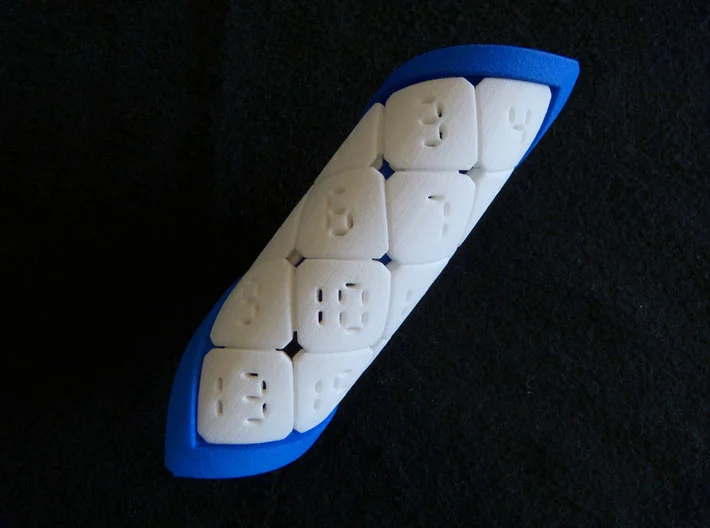
\includegraphics[scale=0.3]{./Figures/coiled15puzzle}
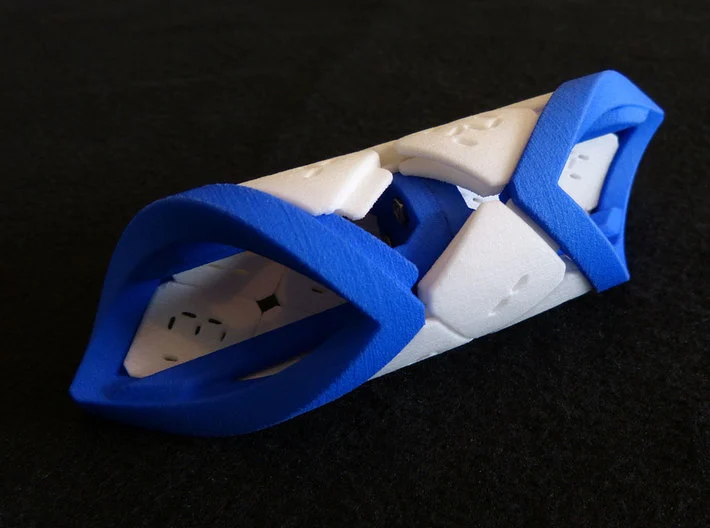
\includegraphics[scale=0.3]{./Figures/coiled15puzzle2.png}
\decoRule
\caption[Coiled 15-puzzle]{Coiled 15-puzzle}
\end{figure}




It is rather easy to see why this is the case, let us discuss why: given a configuration c of the tiles, let us define the permutation p(c) of this configuration according to the following schema: we enumerate the tiles row by row (top to bottom), left to right for odd rows and right to left for the even rows, ignoring the empty compartment. For instance, the following 15-puzzle c:

\begin{fifteen}
\setrow{4}{1,6,2,3}
\setrow{3}{5,10,7,4}
\setrow{2}{9,15,\red14\black,\blue11}
\setrow{1}{13,12,,\blue 8}
\end{fifteen}
\\
\\
we have p(c) = (1, 6, 2, 3, 4, 7, 10, 5, 9, 15, \red 14 \black, \blue 11, 8\black, 12, 13).
\\
It is easy to see that the parity of p(c) cannot change by a legal move of the puzzle. Indeed, p(c) is clearly invariant by lateral move of a tile, so its parity is invariant too. A vertical move of a tile will displace a number in p(c) by an even number of positions right or left. For instance, moving tile 14 into the empty compartment below it results in a new configuration $c_{2}$:

\begin{fifteen}
\setrow{4}{1,6,2,3}
\setrow{3}{5,10,7,4}
\setrow{2}{9,15,,\blue11}
\setrow{1}{13,12,\red14\black,\blue8}
\end{fifteen}
\\
\\
with $p(c_{2})$ = (1, 6, 2, 3, 4, 7, 10, 5, 9, 15, \blue11, 8\black, \red14\black, 12, 13), which is equivalent to moving 14 by 2 positions on the right. This obviously cannot change the parity since exactly 2 pairs of numbers are now in a different order, that is (14, 11) and (14, 8) now appear in the respective opposite orders as (11, 14) and (8, 14).
\\
\\
This is the crux of the proof of the well known necessary condition (even parity of p(c)) for a configuration c to be solvable (see part I of \cite{Johnson1879}).
\\
\\
In the case of the coiled puzzle, we can clearly solve all configurations of even parity, since all the legal moves of the normal puzzle are allowed. In addition, we can for instance transition between the following 2 configurations, which clearly have respectively even and odd parities:

\begin{fifteen}
\centering
\setrow{4}{\red1\black,2,3,4}
\setrow{3}{5,6,7,8}
\setrow{2}{9,10,11,12}
\setrow{1}{13,14,15,}
\end{fifteen}
%
\begin{fifteen}
\setrow{4}{,2,3,4}
\setrow{3}{5,6,7,8}
\setrow{2}{9,10,11,12}
\setrow{1}{13,14,15,\red1\black}
\end{fifteen}
\\
\\
Since it is possible to reach an odd parity configuration, we conclude by invoking symmetry arguments that we can solve all $16!$ configurations. 


%-----------------------------------
%	SUBSECTION 1.2
%-----------------------------------
\subsection{Search Space \& Solvability}

In this thesis, as well as in the code base (\cite{FB}) I have written to do this project, we will consider the general case of a board with n columns and m rows, where $(n, m) \in {\mathbb{N}^{+}}^{2}$, forming $n * m$ compartments. $n * m - 1$ tiles, numbered 1 to $n * m - 1$ are placed in all the compartments but one (which is left empty), and we can slide a tile directly adjascent to the empty compartment into it. Notice from a programming and mathematical analysis perspective, it is often easier to equivalently think of the empty compartment being moved into (or swapped with) an adjacent tile. Starting from a given shuffling of the tiles on the board, our goal will be to execute moves until the tiles in ascending order: left to right, top to bottom (in the usual western reading order), the empty tile being at the very bottom right.
\\
\\
Note that the case where either n or m is 1 is uninteresting since we can only solve the puzzle if the tiles are in order to start with. For instance, in the (n, 1) case, we can only solve n of the $\frac{n!}{2}$ possible configurations. We will therefore only consider the case where both n and m are strictly greater than 1.




%-----------------------------------
%	SUBSECTION 1.3
%-----------------------------------
\subsection{Optimal Cost \& God's Number}

Let us fix n and m, integers strictly greater than 1 and call $\mathcal{C}_{(n, m)}$ the set of all $\frac{(n * m)!}{2}$ solvable configurations of the n by m sliding-puzzle. For any $c \in \mathcal{C}_{(n, m)}$ we define the optimal cost $\mathcal{O}(c)$ to be the minimum number of moves among all solutions for c. Finally we define $\mathcal{G}(n, m)$, God's number for the n by m puzzle as  $\mathcal{G}(n, m) = \max_{c \in \mathcal{C}_{(n, m)}} \mathcal{O}(c)$. Note that since $\frac{(n * m)!}{2}$ grows rather quickly with n and m, it is impossible to compute $\mathcal{G}$ except in rather trivial cases.
\\
\\
A favourite past time among computer scientists around the glove is therefore to search for more refined lower and upper bounds for $\mathcal{G}(n, m)$, for ever increasing values of n and m. For moderate n and m, we can actually solve optimally all possible configurations of the puzzle and compute exactly $\mathcal{G}(n, m)$  (using for instance $A^{*}$ and an admissible heuristic (recall \ref{GSH}, and we shall see modest examples of that in the results section later). For larger values of n and m (say 5 by 5), we do not know what the God number is. Usually, looking for a lower bound is done by \textit{guessing} hard configurations and computing their optimal path via an optimal search. Looking for upper bounds is done via smart decomposition of the puzzle into disjoint nested regions and for which we can compute an upper bound easily (either by combinatorial analysis or via exhaustive search). See for instance \cite{KarlemoOstergard} for an upper bound of 210 on $\mathcal{G}(5, 5)$.
\\
\\
A very poor lower bound can be always obtained by the following reasoning: each move can at best explore three new configurations (4 possible moves at best if the empty tile is not on a border of the board (less if it is): left, right, up, down but one of which is just going back to an already visited configuration). Therefore, after $p$ moves, we would span at best $\mathcal{S}(p) = \frac{3^{p+1} - 1}{2}$ configurations. A lower bound can thus be obtained for $\mathcal{G}(n, m)$ by computing the smallest integer $p$ for which $\mathcal{S}(p) \ge \frac{(n * m)!}{2}$


%-----------------------------------
%	SECTION 2
%-----------------------------------
\section{Rubiks' Cube}

blabla


% Chapter Template

\chapter{Code} % Main chapter title

\label{Chapter3} % Change X to a consecutive number; for referencing this chapter elsewhere, use \ref{ChapterX}

%----------------------------------------------------------------------------------------
%	SECTION 1
%----------------------------------------------------------------------------------------

%\section{Code organisation}

The code I have developed for this project is all publicly available on my github page (\cite{FB}). It can easily be installed using the setup file provided, which makes it easy to then use Python's customary import command to play with the code.
The code is organised in several sub modules and makes use of factories in plenty of places so that I can easily try out different puzzles, dimensions, search techniques, heuristics, network architecture, etc... without having to change anything except the parameters passed in the command line. Here is a visual overview of the code base with the main dependencies between the main submodules and classes. Solid arrows indicate inheritance (e.g. AStar inherits from SearchStrategy), while dotted lines indicate usage (e.g. AStar uses Heuristic, DeepReinforcementLearner uses DeepLearning, etc..).

\begin{landscape}
\begin{figure}[H]
\centering
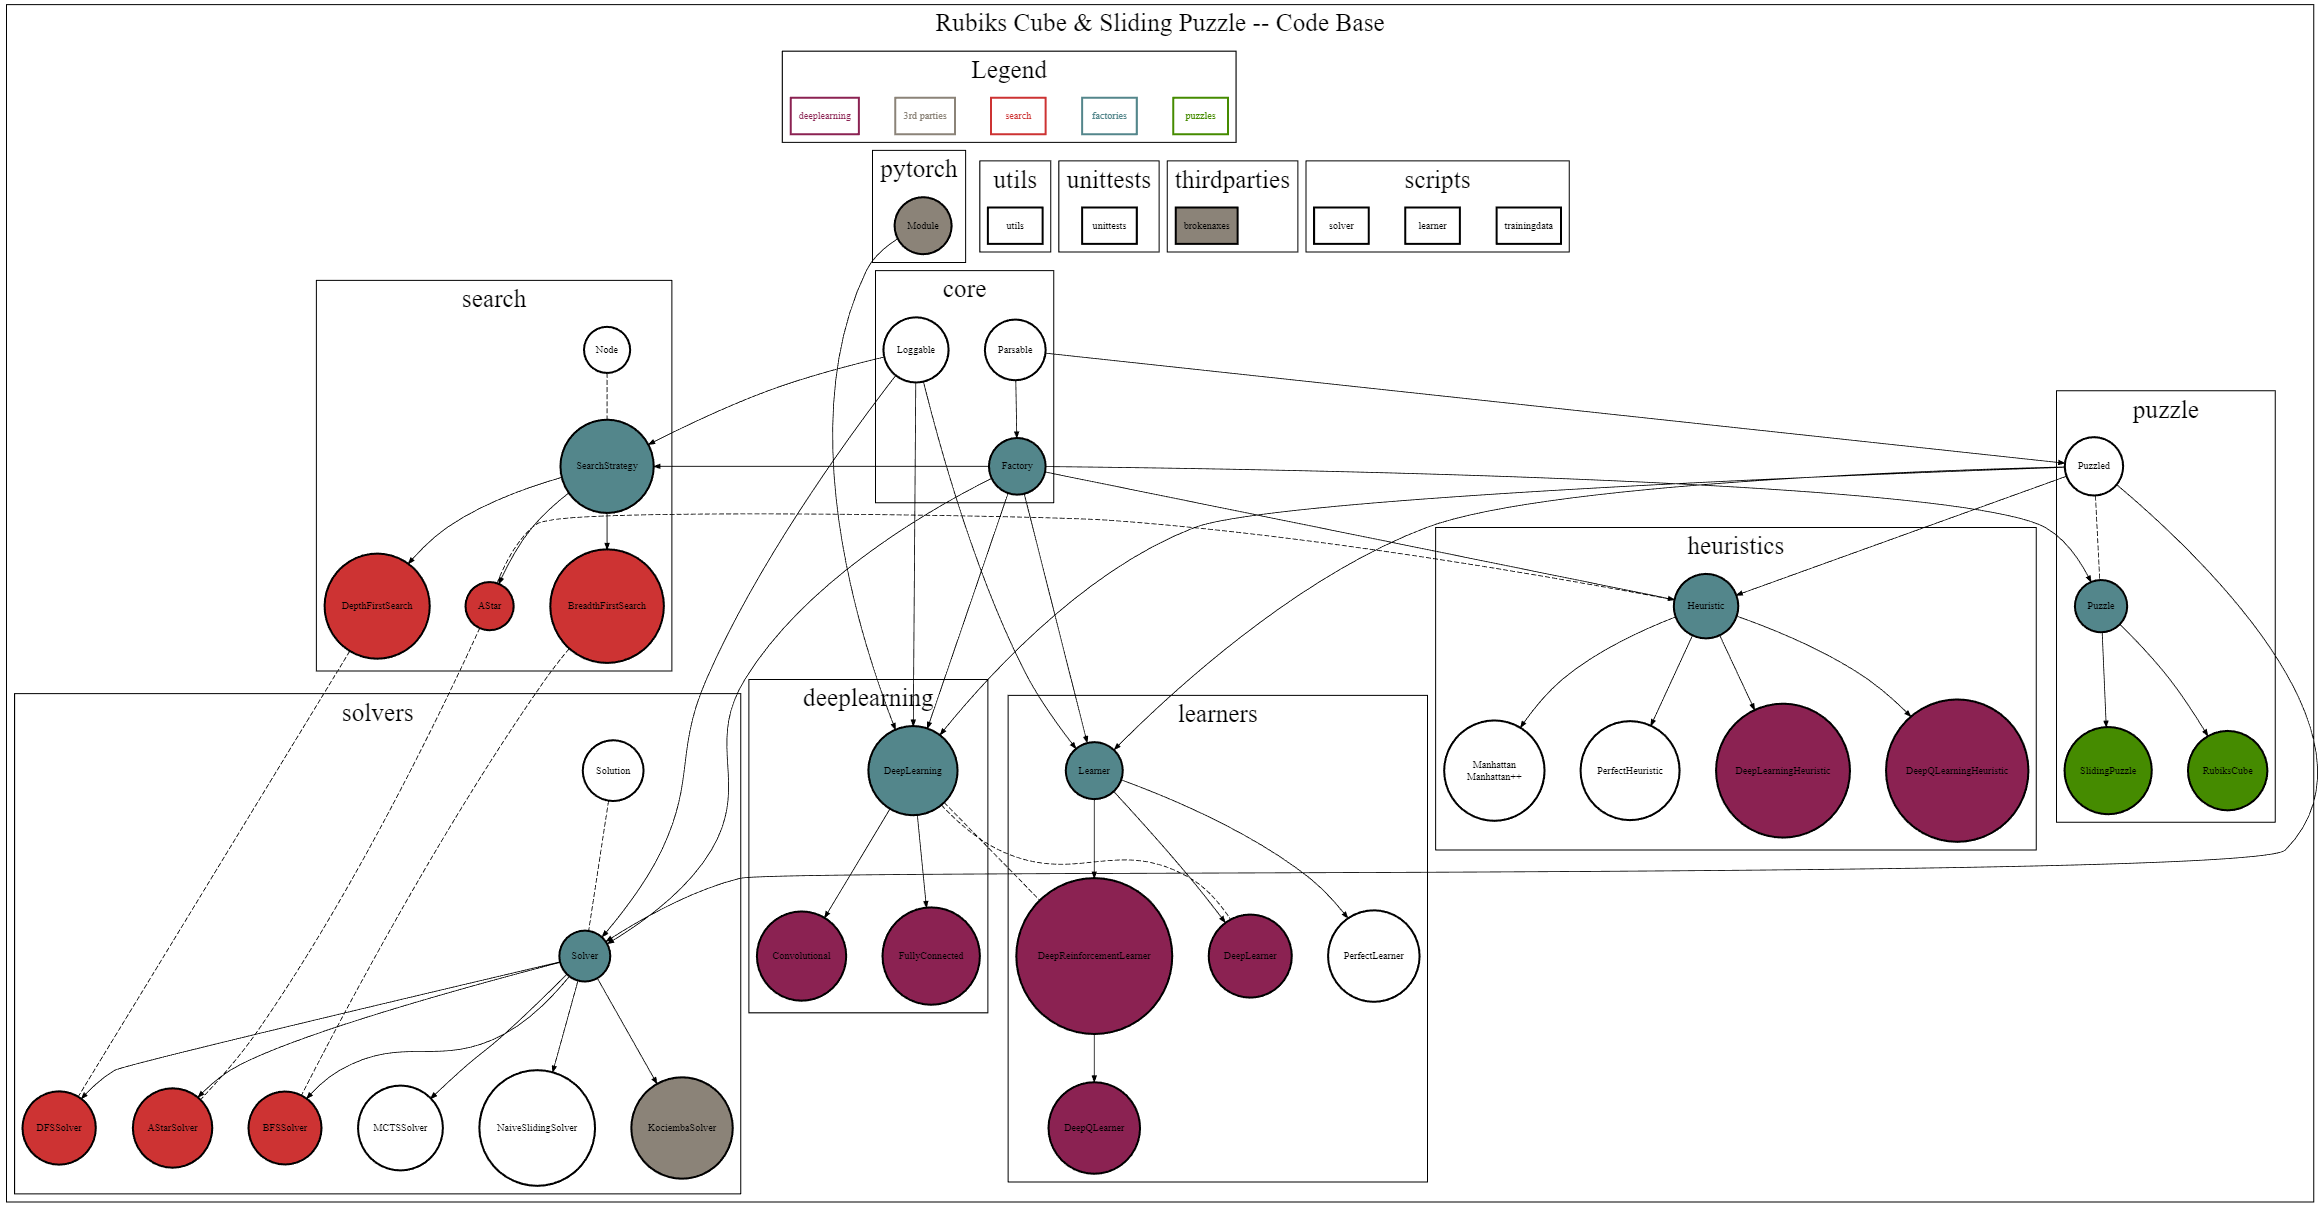
\includegraphics[scale=0.49]{./Figures/codebase}
%\decoRule
\caption[Codebase]{Code base}
\label{fig:Codebase}
\end{figure}
\end{landscape}


Let me now describe what each submodule does in more details:

\section{rubiks.core}
\begin{figure}[H]
\centering
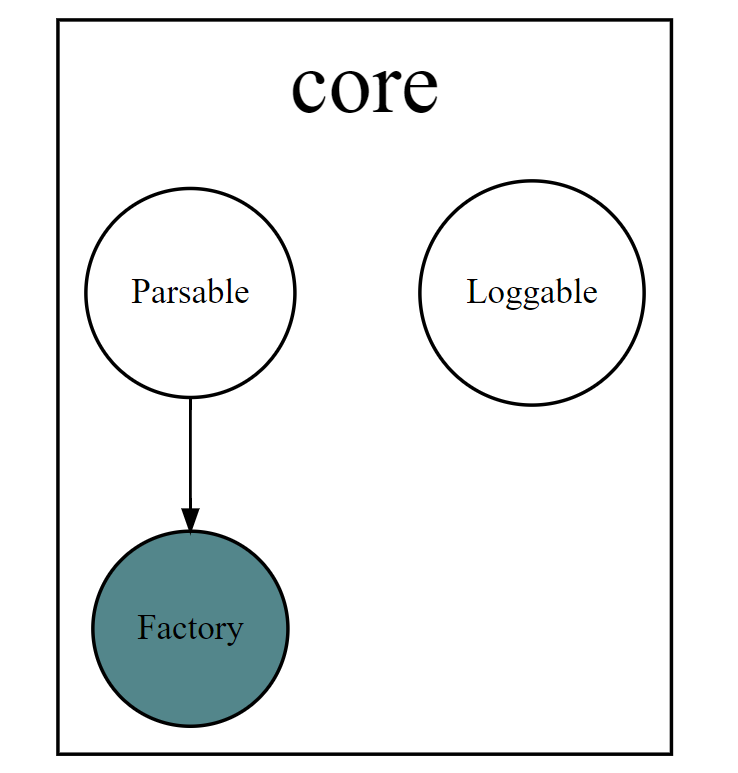
\includegraphics[scale=0.25]{./Figures/codebasecore}
%\decoRule
\caption[Codebase]{rubiks.core}
\label{fig:Codebasecore}
\end{figure}
This submodule contains base classes that make the code base easier to use, debug, and extend. It contains the following:
\begin{itemize}
\item \textbf{Loggable}: a wrapper around Python's logger which automatically picks up classes' names at init and format things (dict, series and dataframes in particular) in a nicer way.
\item \textbf{Parsable}: a wrapper around ArgumentParser, which allows to construct objects in the project from command line, to define dependencies between object's configurations and to help a bit with typing of configs. The end result is that you can pretty much pass **kw\_args everywhere and it just works.
\item \textbf{Factory}: a typical factory pattern. Concrete factories can just define what widget they produce and the factory will help construct them from **kw\_args (or command line, since Factory inherits from Parsable)
\end{itemize}

\section{rubiks.puzzle}
\begin{figure}[H]
\centering
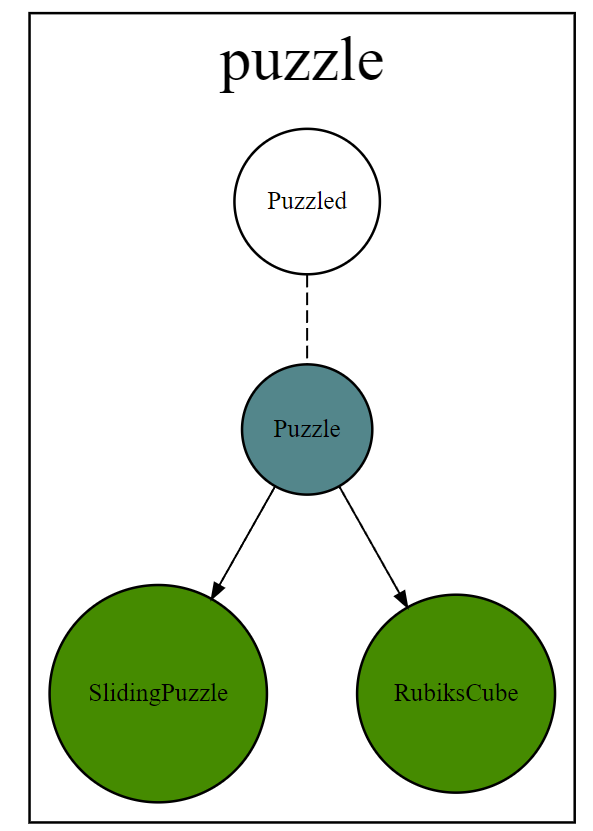
\includegraphics[scale=0.25]{./Figures/codebasepuzzle}
%\decoRule
\caption[Codebase]{rubiks.puzzle}
\label{fig:Codebasepuzzle}
\end{figure}
This submodule contains:
\begin{itemize}
\item \textbf{Puzzle}: a Factory of puzzles. It defines states and actions in the abstract, and provides useful functions to apply moves, shuffle, generate training sets, tell if a state is the goal, etc. Puzzle can manufacture the two following types of puzzles:
\item \textbf{SlidingPuzzle}. Implements the states and moves of the sliding puzzle.
\item \textbf{RubiksCube}. Implements the states and moves of the Rubik's cube.
\\
\\
In addition, this module contains a \textbf{Puzzled} base class which most classes below inherit from. That allow e.g. heuristics, search algorithms, solvers and learners to know what puzzle and dimension they operate on, without having to reimplement these basic facts in each of them.
\end{itemize}

\section{rubiks.search}
\begin{figure}[H]
\centering
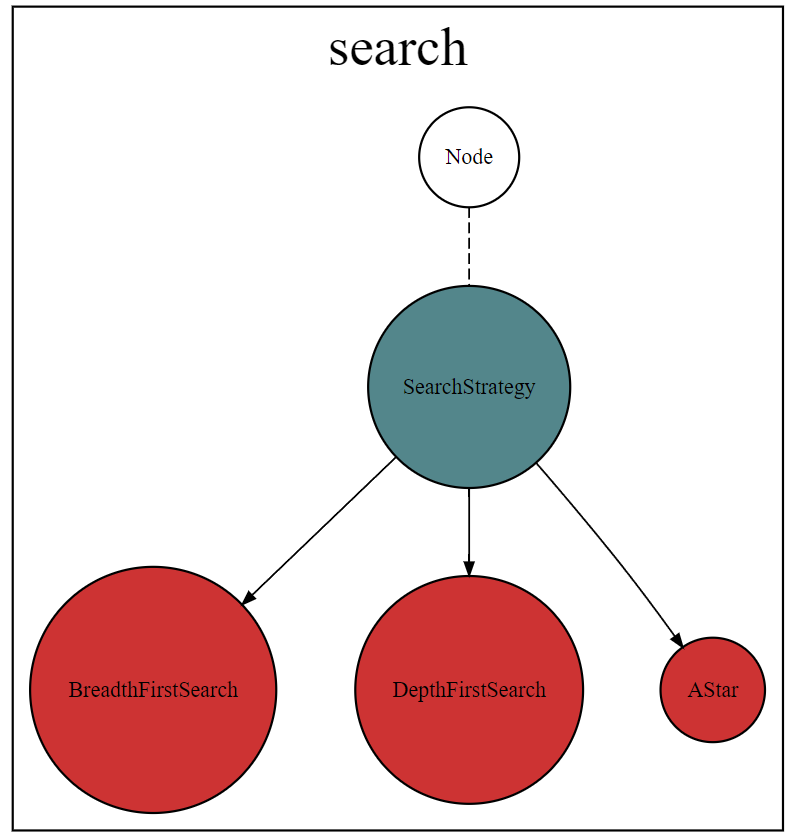
\includegraphics[scale=0.25]{./Figures/codebasesearch}
%\decoRule
\caption[Codebase]{rubiks.search}
\label{fig:Codebasesearch}
\end{figure}
This modules contains graph search strategies. I have actually reused the code I implemented for one of the AIPnT assignments here. It contains the following classes:
\begin{itemize}
\item \textbf{Node}: which contains the state of a graph, as well as link to the previous (parent) state, action that leads from the latter to the former and the cost of the path so far.
\item \textbf{SearchStrategy}, a Factory class which can instantiate the following three types of search strategies to find a path to a goal:
\item \textbf{BreadthFirstSearch}, which is obviously an optimal strategy, but not particularly efficient.
\item \textbf{DepthFirstSearch}, which is not an optimal strategy, and also generally not particularly efficient.
\item \textbf{AStar}, which is optimal, and as efficient as the heuristic it makes use of is.
\end{itemize}

\section{rubiks.heuristics}
\begin{figure}[H]
\centering
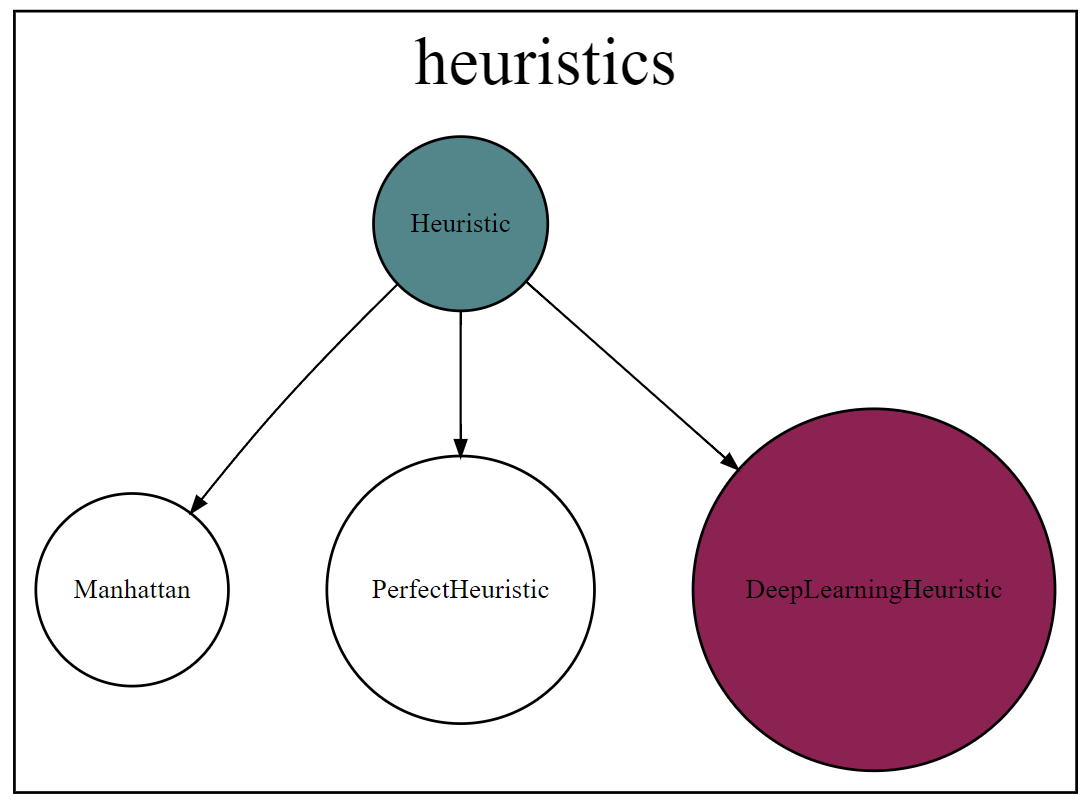
\includegraphics[scale=0.25]{./Figures/codebaseheuristics}
%\decoRule
\caption[Codebase]{rubiks.heuristics}
\label{fig:Codebaseheuristics}
\end{figure}
\label{HSS}
This module contains base class Heuristic, also a Factory. Heuristic can instantiate the following heuristics, which we can use in the AStar strategy from the previous section:
\begin{itemize}
\item \textbf{Manhattan}: This heuristic is specific to the SP. It simply adds for each tile (other than the empty tile) the $L_{1}$ distance between their current position and their target position. We can quickly see that this heuristic is admissible. Indeeed, each move in the SP moves one (and one only) tile by one position. In other puzzles, it is generally the case that a move will affect the position of many tiles (e.g. RC). Therefore, if tiles could somehow freely move on top of one-another (that is, we remove the constraint that there can be at most one tile per compartment, the number of moves necessary to solve the SP would exactly be the Manhattan distance.
\\
\\
The reason why it is interesting to have a known admissible heuristic is that we can obvioulsy compare other heuristics (DL, DRL, DQL, etc) in terms of optimality.
\\
\\
I have also implemented an improvement to the Manhattan distance, which I shall call Manhattan++ in here (and in code logs and graphs) and can be activated by simply passing \textit{plus=True} to the Manhattan Heuristic (see example \ref{ASSS} as well as a thorougher performance comparison on the (n=2, m=5) SP in \ref{MHComp}). It is based on the concept of linear constraints that I read about in lecture notes from Washington University (\cite{SlidingPuzzleLectureNotes}). The idea is simply that when tiles are already placed on their target row or column, but not in the expected order, we will need to get the tiles out of the way of one another to get to the goal state, and this is not accounted for by the Manhattan distance. For instance, in the following (n=2, m=3) SP, the Manhattan distance does not account for the fact that, at best, tile \red 3 \black needs to get out of the way for tiles \blue 1 \black and \blue 2 \black to move, and then needs to get back in its row, adding a cost of 2 to the Manhattan distance.

\begin{center}
\begin{five}
\setrow{2}{\red 3, \blue 1, \blue 2}
\setrow{1}{4, 5, 0}
\end{five}
\end{center}

Two important things to notice are that linear constraints across rows and columns (which I might generically refer to as \textit{lines} in the following) can to be added without breaking admissibility (hence giving more pessimistic, or accurate, cost estimates than simple Manhattan). This is because if a tile is involved in two linear constraints, it will need to get out of the way both horizontally and vertically. The second thing is that when several pairs in a line are not in order, we cannot simply add 2 for each distinct out-of-order pair, the right penalty to add is more subtle than that and needs to be computed recursively. For instance, let us now consider the following configuration:
\begin{center}
\begin{five}
\setrow{2}{\red 3, \red 2, \red 1}
\setrow{1}{4, 5, 0}
\end{five}
\end{center}
The correct penalty to add is not 6 (3 times 2 since all pairs (1, 2), (1, 3) and (2, 3) are out of order, but only 4. Indeed if, say, tile 3 got somehow out of the way at the back of the SP (imagine just another dimension there where we can move tiles) and tile 2 got out of the way by moving down to let tile 1 pass across, we could be done by simply adding 4 to the Manhattan distance (2 to move tile 3 out and back, and 2 to move tile 2 out and back). The correct way to compute the penalty cost for linear constraints is therefore to do it recursively, taking the minimum additional cost of moving either left-most or right-most tile of the line under consideration out of the way (that additional cost to move these left-most or right-most tile is 2 if not at their expected order in the line, 0 otherwise) plus the penalty of reordering the rest of the line.
\\
\\
Finally, as suggested by the reference lecture notes (which give very vague details about the above subtleties), I have precomputed all the penalties for all possible rows, columns and all possible tiles ordering they could have and saved the corresponding penalties in a database. For memory efficiency, I also only saved penalties which are non-zero. The very first time any call to Manhattan++ is made, for a given dimension (n, m), the appropriate data base is computed and populated.
\\
\\
Notice that for an (n, m) SP, there are n rows, each of which can have $\frac{(n * m)!}{(n * m - m)!}$ different ordering of tiles and m columns which can have n columns, each can have $\frac{(n * m)!}{(n * m - n)!}$ different ordering of tiles. This means the pre-computations and data-base sizes for the Manhattan++ heuristic are actually manageable, as it grows much slower than the number of possible puzzles. The maximum number of penalties to compute for $(n, m) \leq (5, 5)$ are:


\begin{center}
\begin{tabular}{l*{6}{c}r}
n              & m & 2 & 3 & 4 & 5\\
\hline
2              &   & 48 & 330 & 3,584 & 60,930 \\
3              &   &   & 3,024  & 40,920 &  1,094,730  \\
4              &   &   &  & 349,440 & 8,023,320   \\
5              &   &   &  &  & 63,756,000   \\
\end{tabular}
\end{center}
Taking also into account that we only store non-zero penalties, we actually get the following (quite smaller) number of penalties in our data bases:
\begin{center}
\begin{tabular}{l*{6}{c}r}
n              & m & 2 & 3 & 4 & 5\\
\hline
2              &   & 2 & 46 & 1,238  & 32,888 \\
3              &   &  & 278  & 7,122 & 328,894   \\
4              &   &   &  & 40,546 &  1,456,680 \\
5              &   &   &  &  &  8,215,382 \\
\end{tabular}
\end{center}



\item \textbf{PerfectHeuristic}: this reads from a data base the optimal costs, pre-computed by the PerfectLearner (see below \ref{PLcode})
\item \textbf{DeepLearningHeuristic}: this uses a network which has been trained using DRL by the DeepReinforcementLearner (see below \ref{DRLcode})
\end{itemize}



\section{rubiks.deeplearning}
\begin{figure}[H]
\centering
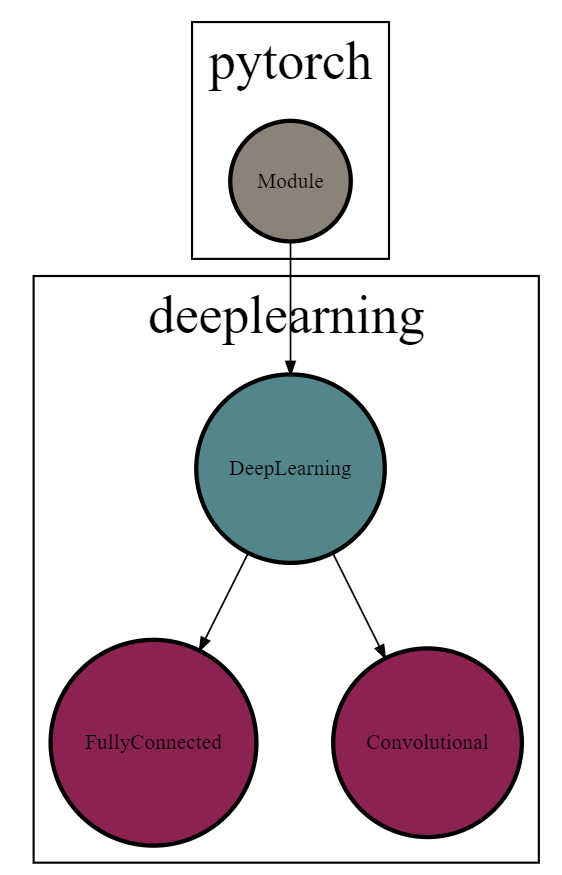
\includegraphics[scale=0.25]{./Figures/codebasedeeplearning}
%\decoRule
\caption[Codebase]{rubiks.deeplearning}
\label{fig:Codebasedeeplearning}
\end{figure}
This module is a wrapper around Pytorch. It contains:
\begin{itemize}
\item \textbf{DeepLearning}: a Puzzled Loggable Factory that can instantiate some configurable deep networks, and provide the necessary glue with the rest of the code base so that puzzles be seemlessly passed to the networks and trained on. 
\item \textbf{FullyConnected}: wrapper around a Pytorch fully connected network, with configurable hidden layers and size. There are some params as well to add drop out, and to indicate whether or not the inputs are one hot encoding (in which case the first layer is automatically adjusted in size, using information from the puzzle dimension).
\item \textbf{Convolutional}: similar wrapper to FullyConnected, but with the ability to add some parallel convolutional layers to complement fully connected layers.
\end{itemize}


\section{rubiks.learners}
\label{sec:codelearners}
\begin{figure}[H]
\centering
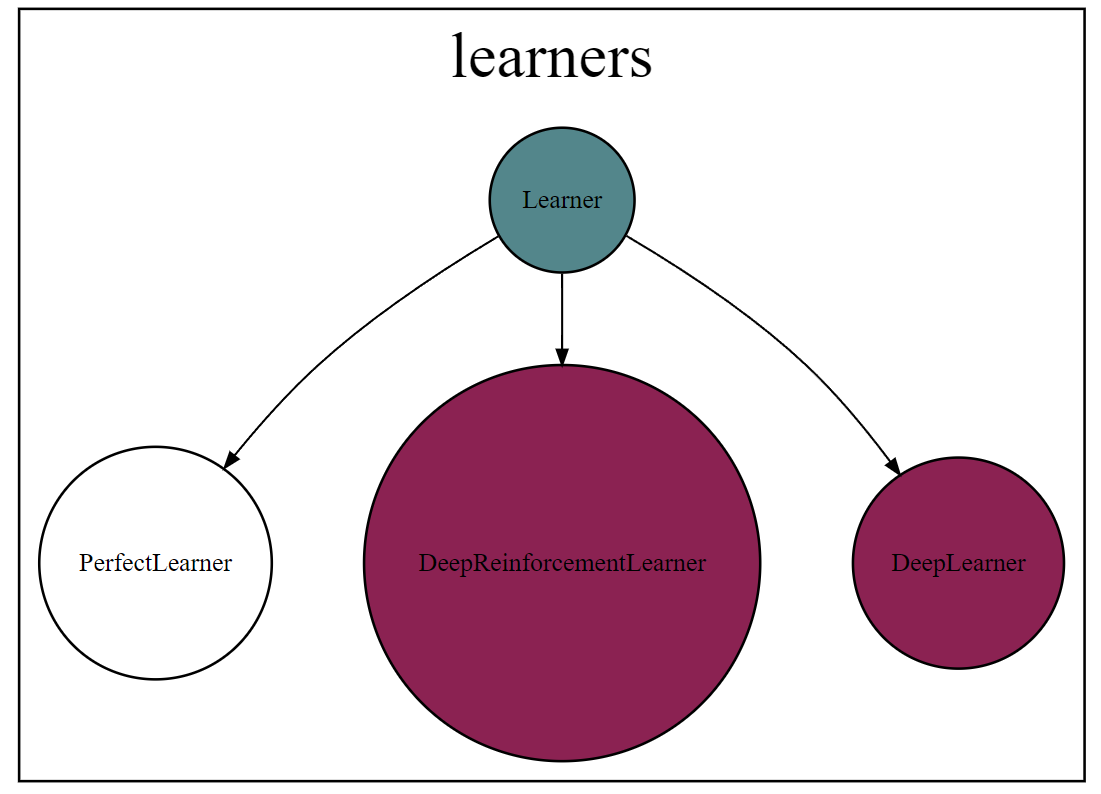
\includegraphics[scale=0.25]{./Figures/codebaselearners}
%\decoRule
\caption[Codebase]{rubiks.learners}
\label{fig:Codebaselearners}
\end{figure}
\label{PLcode}
\label{DRLcode}
This module implements learners, which learn something from a puzzle, store what they learnt, and can display interesting things about what they learnt.

\begin{itemize}
\item \textbf{Learner} is a Puzzled Loggable Factory. It provides some common code to learners (to save or purge what they learnt), kick off learning and plot results. Concrete derived implementation define what and how they learn, and what interesting they can display about this learning process. Currently the two implemented learners are:
\item \textbf{PerfectLearner}: It instantiates an optimal solver ($A^{*}$ with a configurable heuristic - but will only accept heuristic that advertise themselves as optimal. The learning consists in generating all the possible configuration of the considered puzzle, solve them with the optimal solver, and save the optimal cost of it as well as those of the whole solution path. The code allows for parallelization, stop and restart so that we can run on several different occasions and keep completing a database of solutions if necessary or desired. Once the PerfectLearner has completed its job, it can display some interesting information, such as the puzzle's God's number, the distribution of number of puzzles versus optimal cost, the hardest configuration it came across, and how long it took it to come up with the full knowledge of that puzzle. I will show in section \ref{PLSS} how to run an example. Notice that for puzzles of too high dimension, where my computing resources will not allow to solve exhaustively all the configurations of a given dimension, this class can still be used to populate a data base of optimal costs, which can then be used by DeepLearner. If it is to be used this way, the PerfectLearner can be configured to use perfectly random configurations to learn from, rather than going through the configurations one by one in a well defined order.

\item \textbf{DeepLearner} tbd
\item \textbf{DeepReinforcementLearner}: It instantiates a DeepLearning (network), and trains it using DRL. It then saves the trained network, which can then be used in the DeepLearningHeuristic we have seen earlier in section \ref{HSS}. The DeepReinforcementLearner runs for a number of epochs (or less if, based on other parameters discussed below, it is deemed to have converged). 


\end{itemize}


\section{rubiks.solvers}
\begin{figure}[H]
\centering
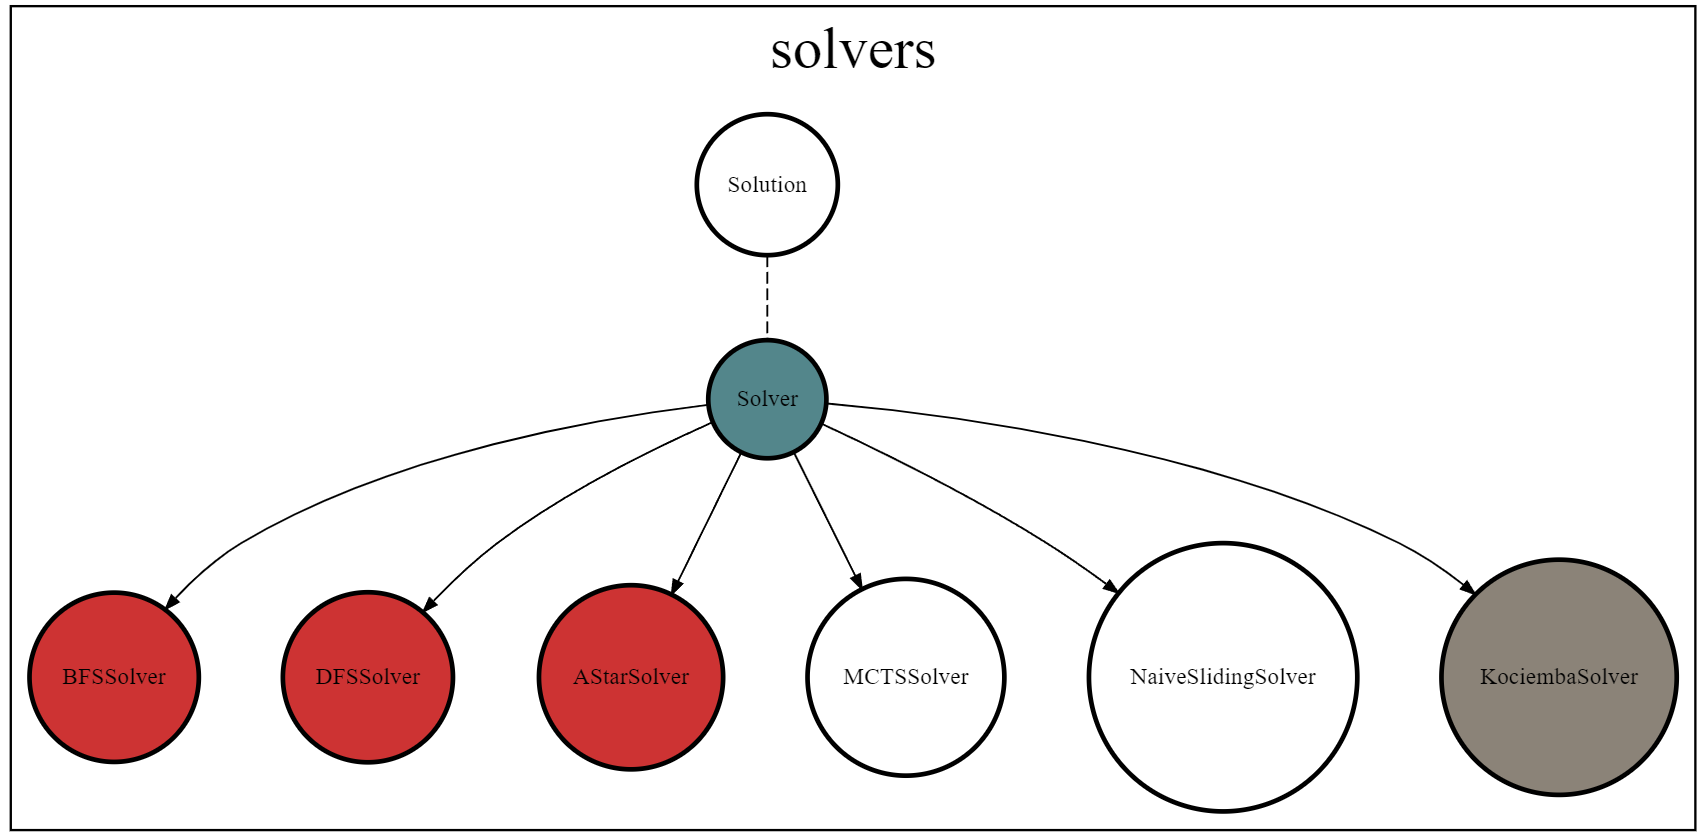
\includegraphics[scale=0.25]{./Figures/codebasesolvers}
%\decoRule
\caption[Codebase]{rubiks.solvers}
\label{fig:Codebasesolvers}
\end{figure}
This module implements solvers, which solve puzzles. The base class Solver is a Factory of solvers, and in addition to being able to instantiating the following types of solvers, can run different solvers through a similal sequences of random puzzles (for various increasing degrees of difficulty (shuffling), and/or perfectly shuffled ones) and display a comparison of how they perform in a number of metrics.

\begin{itemize}
\item \textbf{DFSSolver} TBD
\item \textbf{BFSSolver} TBD
\item \textbf{AStarSolver} TBD
\item \textbf{NaiveSlidingSolver} TBD
\item \textbf{MonteCarloSearchTreeSolver} TBI I want to implement this in August when working on the Rubiks' ... following the Rubik's paper fromMcAleer \& Agostilenni et al \cite{https://doi.org/10.48550/arxiv.1805.07470}
\end{itemize}

\section{rubiks.scripts}

\begin{figure}[H]
\centering
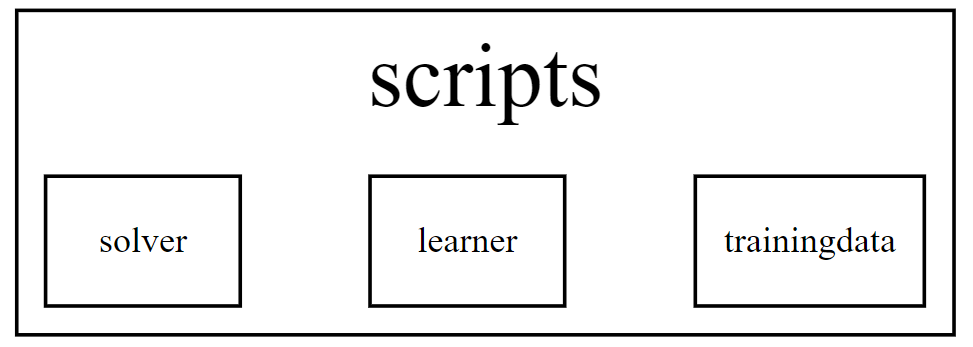
\includegraphics[scale=0.25]{./Figures/codebasescripts}
%\decoRule
\caption[Codebase]{rubiks.scripts}
\label{fig:Codebasescripts}
\end{figure}

Finally it is worth noting that the code will save on disk a lot of data (e.g. the learners will save what they have learnt, e.g. a Pytorch network or a data base of optimal costs, the performance comparison will run solvers versus very many configurations of puzzles and save the results for later being able to display) etc... The base of the tree to save all this data can be chosen by setting up the "RUBIKSDATA" environment variable. If not, it will go somewhere in you HOME :)

% Chapter Template

\chapter{Results - Sliding Puzzle} % Main chapter title

\label{sec:ResultsSP} % Change X to a consecutive number; for referencing this chapter elsewhere, use \ref{ChapterX}





\begin{center}
\begin{tabular}{l*{9}{c}r}
\hline
\textbf{solver}      & & \textbf{Sliding Puzzle} & \textbf{2x2} & \textbf{2x3} & \textbf{2x4} & \textbf{2x5}  & \textbf{3x3} & \textbf{3x4} & \textbf{4x4} \\ 
\hline
BFS   & & & & & & &  x  & & \\
\hline
A$^{*}$[Manhattan]   & & & & & &  x  &  x  & & \\
\hline
A$^{*}$[Manhattan++]   & & & & & &  x  &  x  & & \\
\hline
A$^{*}$[Perfect]   & & &  x  &  x  &  x  &  x  &  x  & & \\
\hline
Naive   & & & & & & &  x  & & \\
\hline
A$^{*}$[DL[A$^{*}$[Perfect]]]   & & & & & & &  x  & & \\
\hline
A$^{*}$[DRL]   & & & & & & &  x  & & \\
\hline
A$^{*}$[DQL]   & & & & & & &  x  & & \\
\hline
MCTS[DQL][c=TBD]   & & & & & & &  x  & & \\
\end{tabular}
\end{center}












%----------------------------------------------------------------------------------------
%	SECTION 1
%----------------------------------------------------------------------------------------

\section{Low dimension}
\label{sec:SPLowDimension}

\subsection{God numbers and hardest puzzles}

As mentioned in chapter \ref{sec:Puzzles}, the state space cardinality for the SP grows very quickly with n and m. Here are the only dimensions which have less than 239.5 millions states. Note I am also only considering n $\leq$ m since (p, q) can always be solved if we know how to solve (q, p):
\\
\\
\begin{center}
\begin{tabular}{l*{6}{c}r}
n              & m & 2 & 3 & 4 & 5\\
\hline
2              &   & 12 & 360 & 20,160 & 1,814,400 \\
3              &   &   & 181,440 &  &    \\
\end{tabular}
\end{center}
In this section, I will discuss \textbf{full} results for these 5 puzzles. In order to fully solve them, one can simply use rubiks.scripts.learner, setting up the PerfectLearner with A* and manhattan heuristic, or instantiate directly a PerfectLearner as have seen in section \ref{PLSS}
I obtained the following God numbers for these puzzles:
\begin{center}
\begin{tabular}{l*{6}{c}r}
n              & m & 2 & 3 & 4 & 5\\
\hline
2              &   & 6 & 21 & 36 & 55* \\
3              &   &   & 31 &  &    \\
\end{tabular}
\end{center}
* provisional result
\\
\\
Notice that among the above dimensions, (n=2, m=5) is the largest and hardest one. I had to run its PerfectLearner over a couple of days, on a c5.18xlarge instance (72 cores) on Amazon EC2.
\\
\\
The perfectLearner also keeps track of (one of) the hardest puzzles it has encountered (i.e. requiring a number of steps equal to their respective God number to solves):
\\
\\
\underline{Most difficult 2x2 (6 moves)}:
\begin{center}
\begin{three}
\setrow{2}{,3}
\setrow{1}{2,1}
\end{three}
\end{center}
\underline{Most difficult 2x3 (21 moves)}:
\begin{center}
\begin{five}
\setrow{2}{4,5,}
\setrow{1}{1,2,3}
\end{five}
\end{center}
\underline{Most difficult 2x4 (36 moves)}:
\begin{center}
\begin{seven}
\setrow{2}{,7,2,1}
\setrow{1}{4,3,6,5}
\end{seven}
\end{center}
\underline{Most difficult 2x5 (55* moves)}:
\begin{center}
\begin{nine}
\setrow{2}{,9,3,7,1}
\setrow{1}{5,4,8,2,6}
\end{nine}
\end{center}
* provisional result
\\
\\
\underline{Most difficult 3x3 (31 moves)}:
\begin{center}
\begin{eight}
\setrow{3}{8,6,7}
\setrow{2}{2,5,4}
\setrow{1}{3,,1}
\end{eight}
\end{center}




\subsection{Manhattan heuristic}
\label{MHComp}
In this section, I verify empirically that, as expected, the overhead of adding penalty in Manhattan++ for the linear constraint (which have all been precomputed and stored in a database) is more than compensated for by the reduction in nodes expansion. I have run my solver script for (n=2, m=5) in performance test mode, for both Manhattan and Manhattan++, with 250 randomly shuffled puzzles with \textit{nb\_shuffles} from 0 to 60 by increment of 5, as well as with \textit{nb\_shuffles = $\inf$}. The resulting run time and nodes expansions are as follows:

\begin{figure}[H]
\centering
\hspace*{-2.5cm}
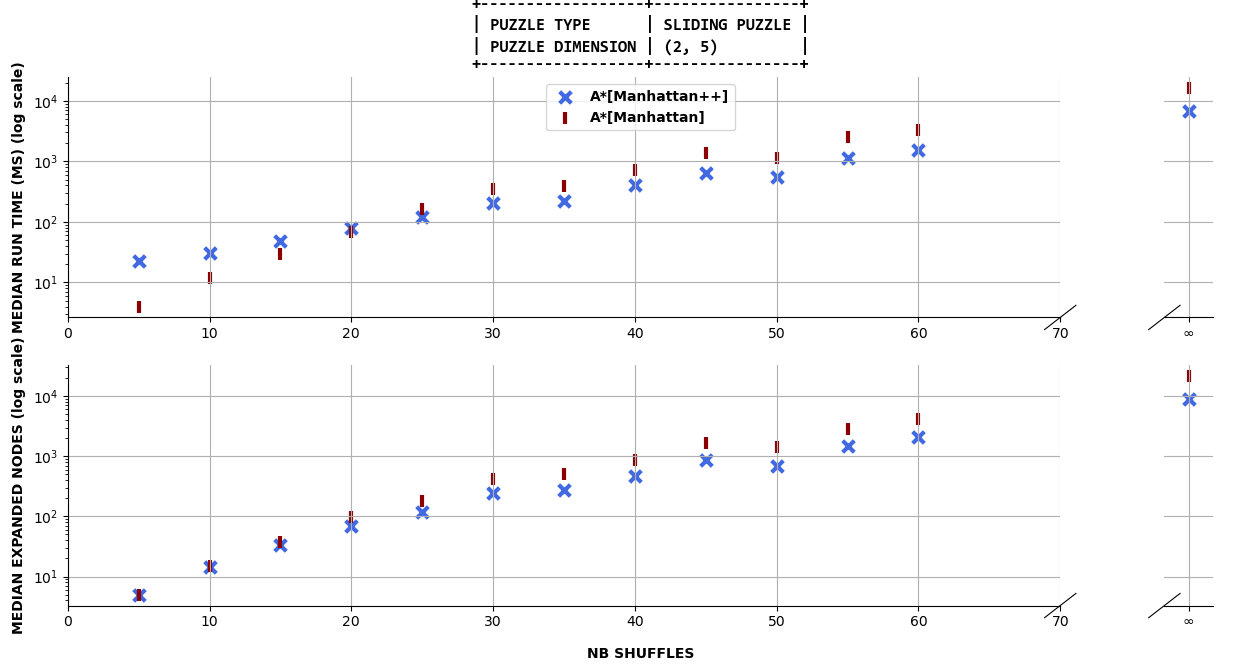
\includegraphics[scale=0.45]{./Figures/25SPPerformanceManhattan}
%\decoRule
\caption[SP]{Manhattan vs Manhattan++}
\label{fig:25SPPerformanceManhattan}
\end{figure}

As can be seen, for low difficulty (up to \textit{nb\_shuffles = 20}), the node expansions are about the same in both cases, and the overhead of adding the linear constraints penalty increases the run time. However, for any non trivial case, Manhattan++ outperforms considerably (by a factor of about 2.5). For the 250 \textit{perfectly} shuffled instances, I got the following:



\begin{center}
\begin{tabular}{l*{7}{c}r}
                              & avg cost  & max cost & avg nodes & max nodes & avg run time (ms) & max run time (ms) \\
\hline
Manhattan                   &  34.7  & 50 & 133,332 & 2,110,887 & 49,561 & 606,838 \\
Manhattan++              & 34.7 &  50 & 53,637 & 962,324 & 19,723 & 239,468 \\
Improvement               & n/a &  n/a & x2.5 & x2.2 & x2.5 & x2.5 \\
\end{tabular}
\end{center}






%-----------------------------------
%	SECTION 2
%-----------------------------------
\section{Intermediary case - 3x3}
\label{sec:S33}


\subsection{Perfect learner}
As discussed in the previous section section \ref{sec:SPLowDimension}, the 3 by 3 SP is one of the cases I have been able to solve perfectly, since it only has 181,440 possible configurations. Its God number is only 31, which definitely makes it manageable. However, this is already an intermediary size, large enough that it is worth trying and comparing a few different methods, including deep reinforcement learning. To start with, I ran the PerfectLearner with n=m=3, and the results are shown below in figure \ref{fig:33SPPerfectLearning}. It is interesting to note that there are only two hardest configurations (cost 31) and 221 configurations of cost 30.


\newgeometry{top=0mm, bottom=0mm, left=0mm, right=0mm}
\begin{landscape}
\centering\vspace*{\fill}
\begin{figure}[H]
\centering
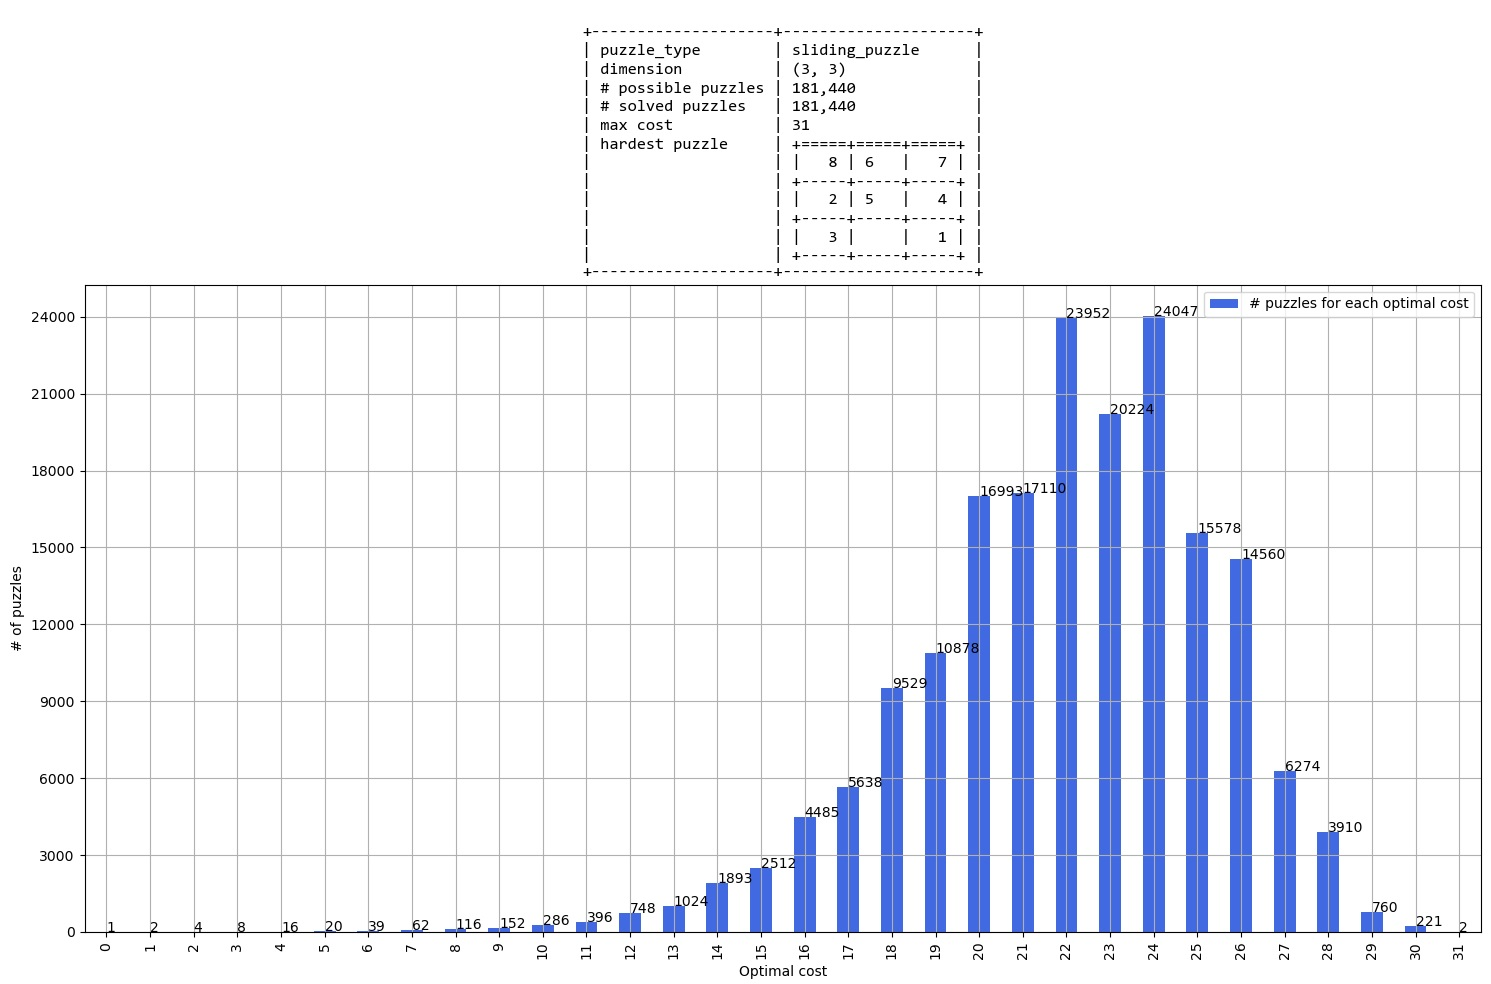
\includegraphics[scale=0.7]{./Figures/33SPPerfectLearning.jpeg}
%\decoRule
\caption[33SPPerfectLearning]{Perfect Learning 3x3 SP}
\label{fig:33SPPerfectLearning}
\end{figure}
\vfill
\end{landscape}
\restoregeometry




\subsection{Deep reinforcement learner}
 The DeepReinforcementLearner's learning is shown in figure \ref{fig:33SPDeepReinforcementLearning}:

\newgeometry{top=0mm, bottom=0mm, left=0mm, right=0mm}
\begin{landscape}
\centering\vspace*{\fill}
\begin{figure}[H]
\centering
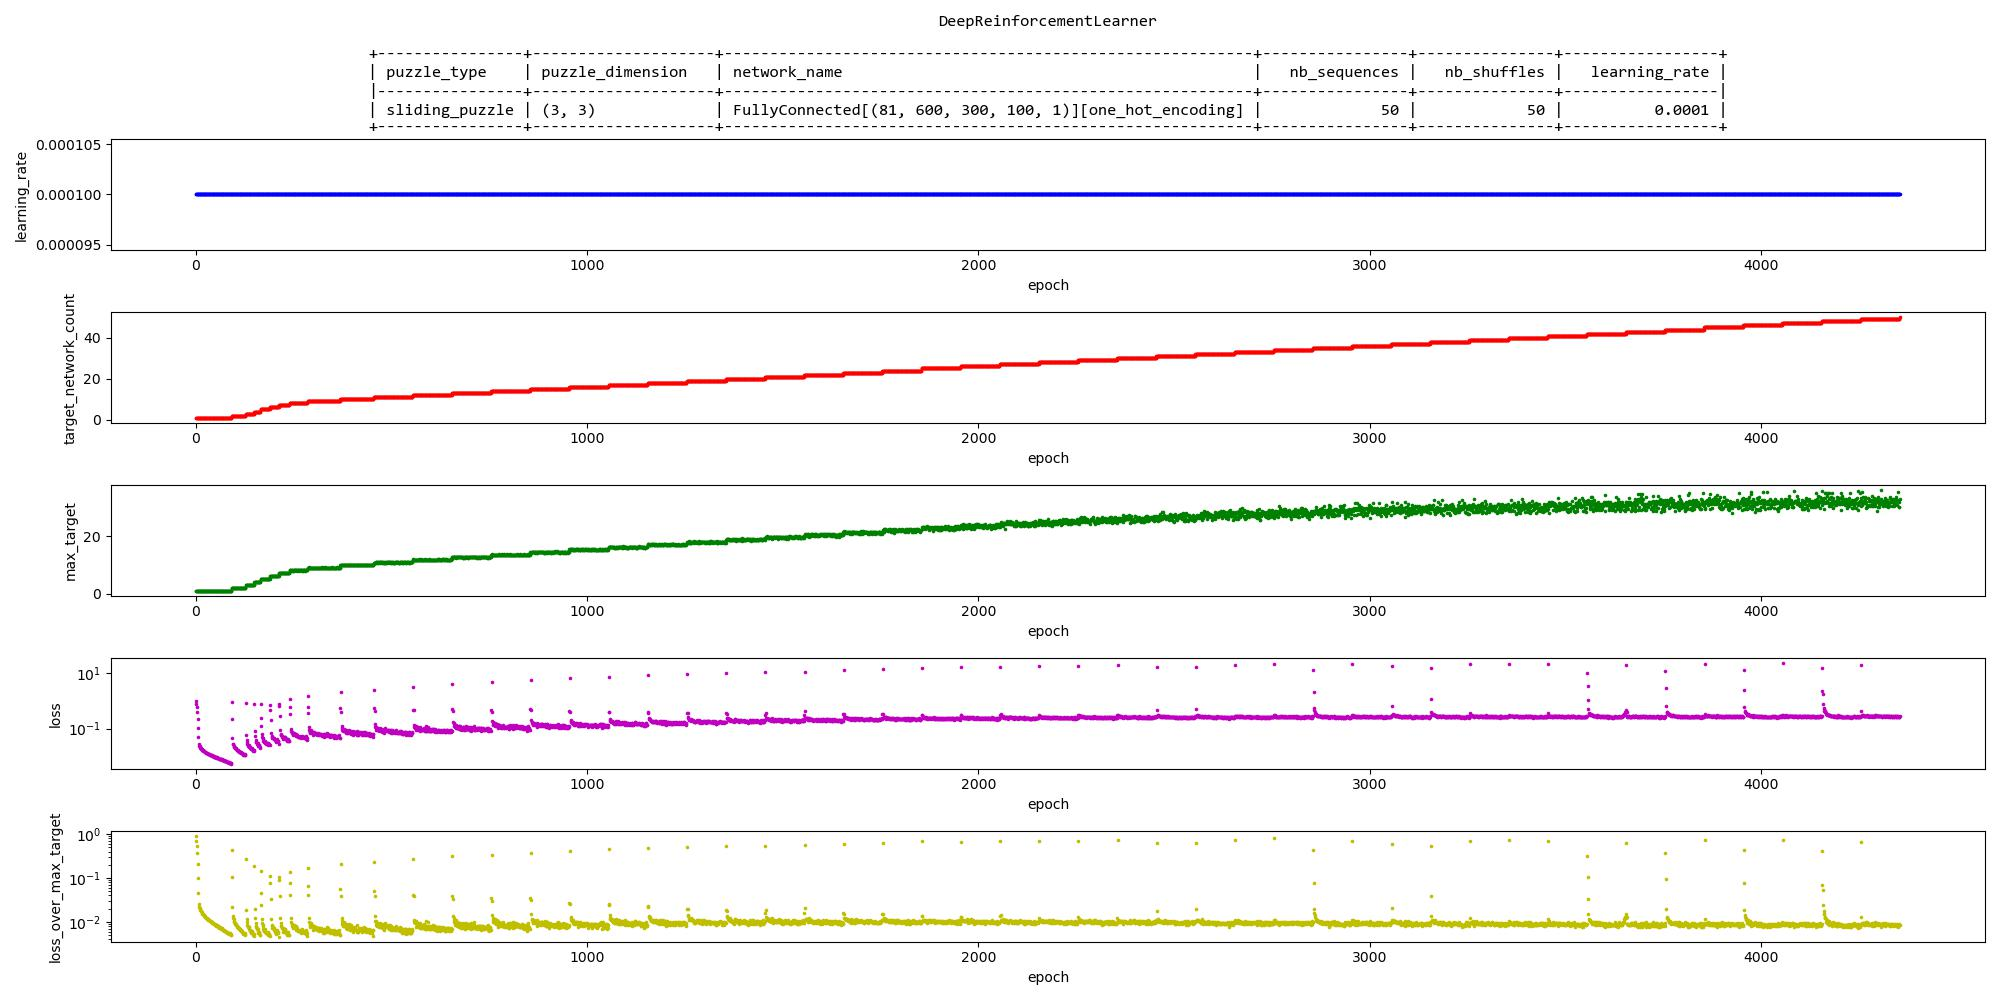
\includegraphics[align=c, scale=0.55]{./Figures/33SPDeepReinforcementLearning}
\caption[33SPDeepReinforcementLearning]{Deep reinforcement learner 3x3 SP}
\label{fig:33SPDeepReinforcementLearning}
\end{figure}
\vfill
\end{landscape}
\restoregeometry



\subsection{DRL vs DQL}


\subsection{MCTS DQL}




\subsection{Solvers' comparison}
\label{ssec:33SPSC}
Let me discuss a comparison of several algorithms on 1000 random puzzles generated for a number of random shuffling (with best-effort-no-backtracking) from 0 to 50 in step of 2, as well as for perfect shuffling (denoted by $\infty$) on the comparison graphs. The results are shown in figure \ref{fig:33SPPerformance}
\\
DL: 100 seq 15 to 31 shuffles 10k epochs connected 600 300 100
\\
Manhattan vs ++
\\
DQL vs DRL
\\
DxL vs Perfect





\newgeometry{top=0mm, bottom=0mm, left=0mm, right=0mm}
\begin{landscape}
\centering\vspace*{\fill}
\begin{figure}[H]
\centering
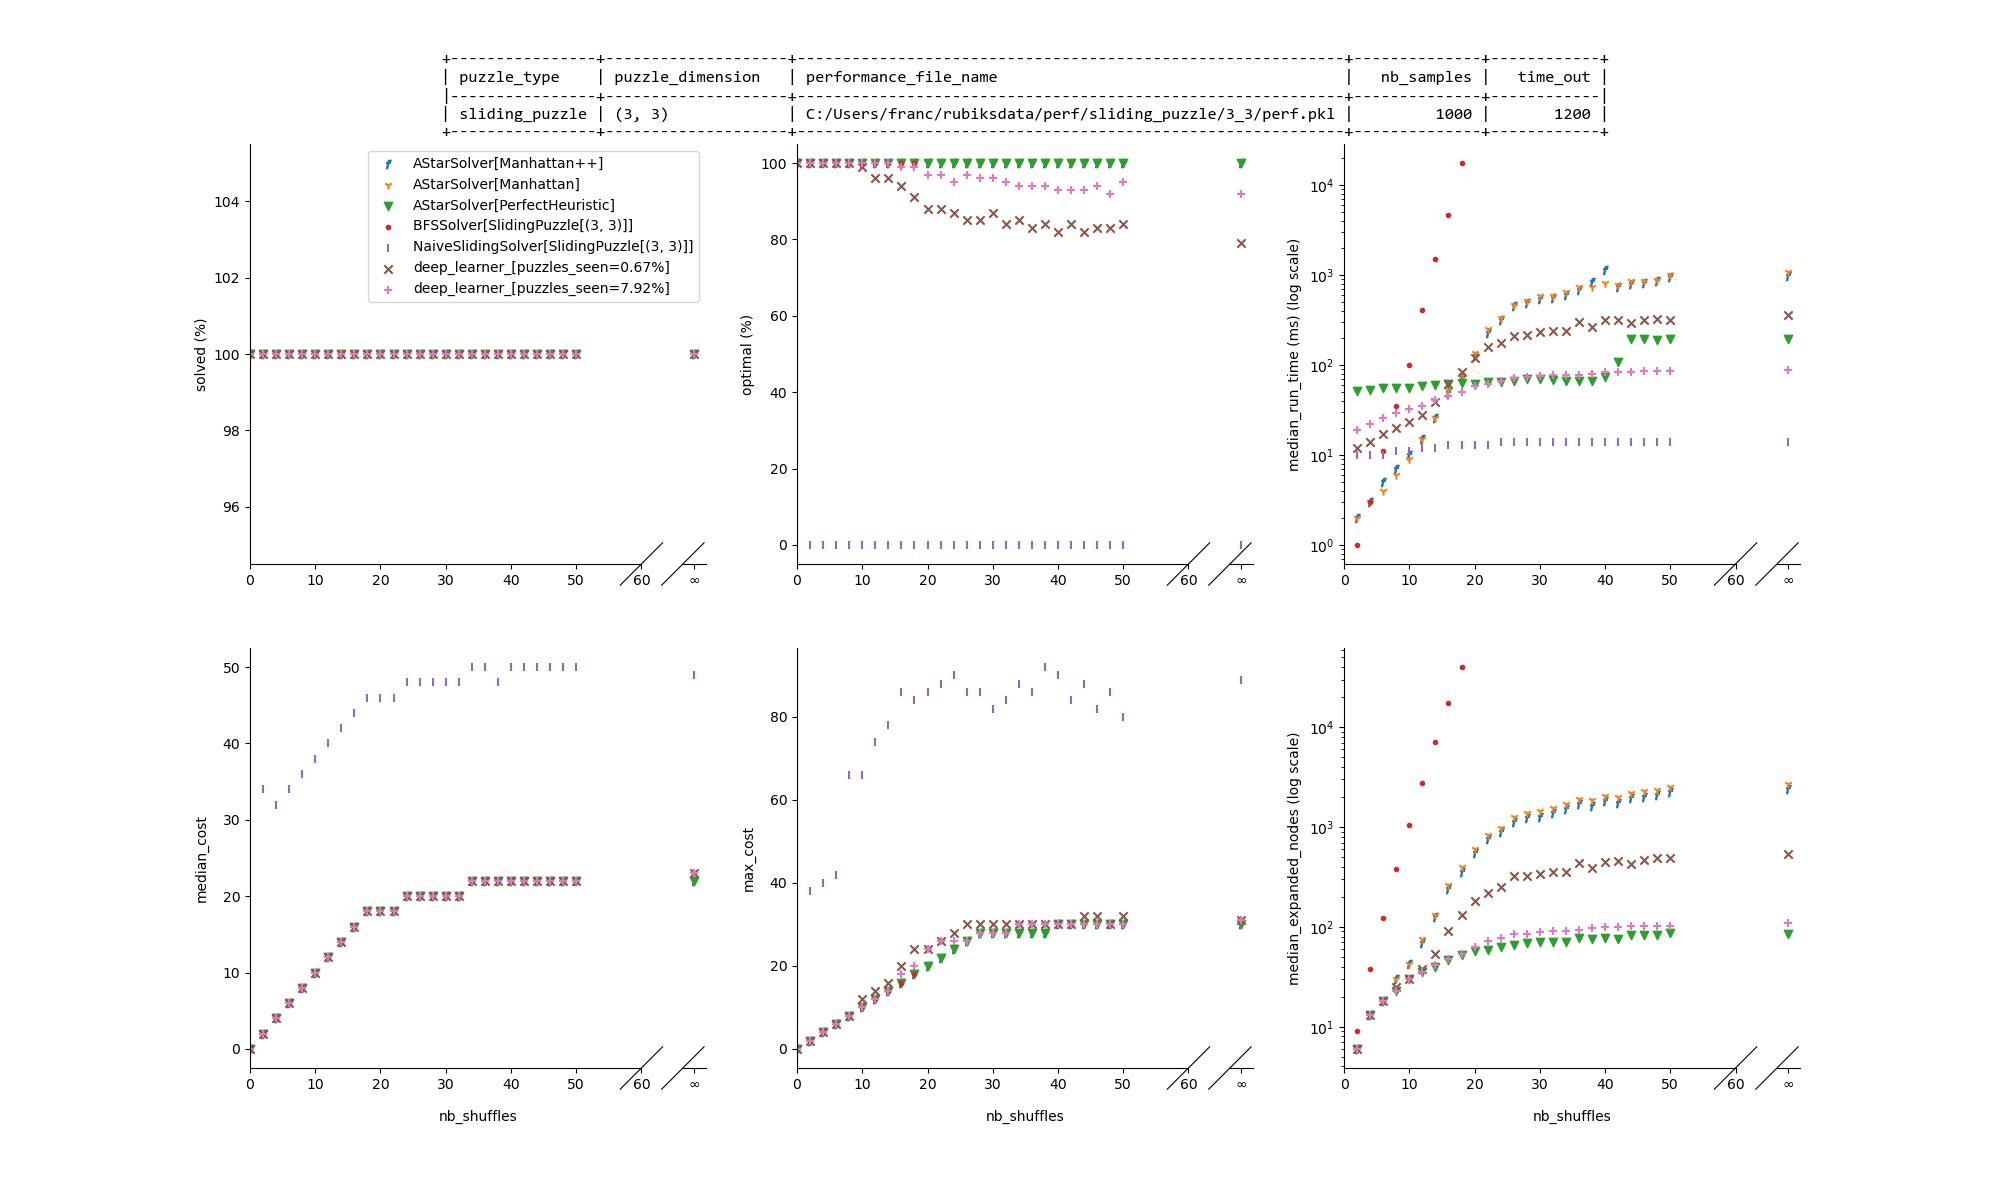
\includegraphics[scale=0.63]{./Figures/33SPPerformance.jpeg}
%\decoRule
\caption[33SPPerformance]{Solvers' performance comparison 3x3 SP}
\label{fig:33SPPerformance}
\end{figure}
\vfill
\end{landscape}
\restoregeometry


\subsection{Solving the hardest 3x3 problem}
To finish with the 3x3 SP, let me try to throw one of the two hardest 3x3 configurations (see subsection \ref{sec:SPLowDimension}) at the different solvers to see how they fare. The results are shown here

\begin{center}
\begin{tabular}{l*{5}{c}r}
\hline
\textbf{solver}      & & \textbf{cost} & \textbf{\# expanded nodes} & \textbf{run time (ms)} \\
\hline
AStarSolver[Manhattan]   &   &      31  & 58,859  & 11,327  \\
\hline
AStarSolver[Manhattan++]   &   &      31  & 34,224  & 7,080  \\
\hline
AStarSolver[PerfectHeuristic]  &   & 31 & 1,585 & 202 \\
\hline
AStarSolver[DRLHeuristic]  &   & 31 & 101 & 58 \\
\hline
MCTSSolver[DQLHeuristic][c=0]  &   & 101 & 103 & 456 \\
\hline
MCTSSolver[DQLHeuristic][c=69]  &   & 35 & 2,244 & 8,873 \\
\hline
BFS  &   & - & - & time out \\
\hline
NaiveSlidingSolver  &   & 61 & n/a & 18 \\
\hline
\end{tabular}
\end{center}
On this specific configuration, there was obviously no chance that the BFS would complete, hence it timed out. It would have no matter what time out I set. Indeed, since it has no heuristic to guide its search, it would need to explore in the order of $3^{31}$ - roughly 617 trillions - nodes to reach the goal!
\\
Rather interestingly, my DRL heuristic performs much better than the manhattan heuristic (not super suprising), but also outperforms the perfect heuristic quite significantly both in terms of run time and of nodes expansion. Obviously there is no guarantee that the perfect heuristic will not be outperformed on some random configuration, and it does on this occasion. However, as we have seen in the previous subection \ref{ssec:33SPSC}, it is not the case on average.
\\
Finally, the naive solver outperforms every other solver in terms of run time, but finds a rather poor solution of 61 moves.



%-----------------------------------
%	SECTION 3
%-----------------------------------
\section{3x4}

\label{ssec:34SPSC}

\newgeometry{top=0mm, bottom=0mm, left=0mm, right=0mm}
\begin{landscape}
\centering\vspace*{\fill}
\begin{figure}[H]
\centering
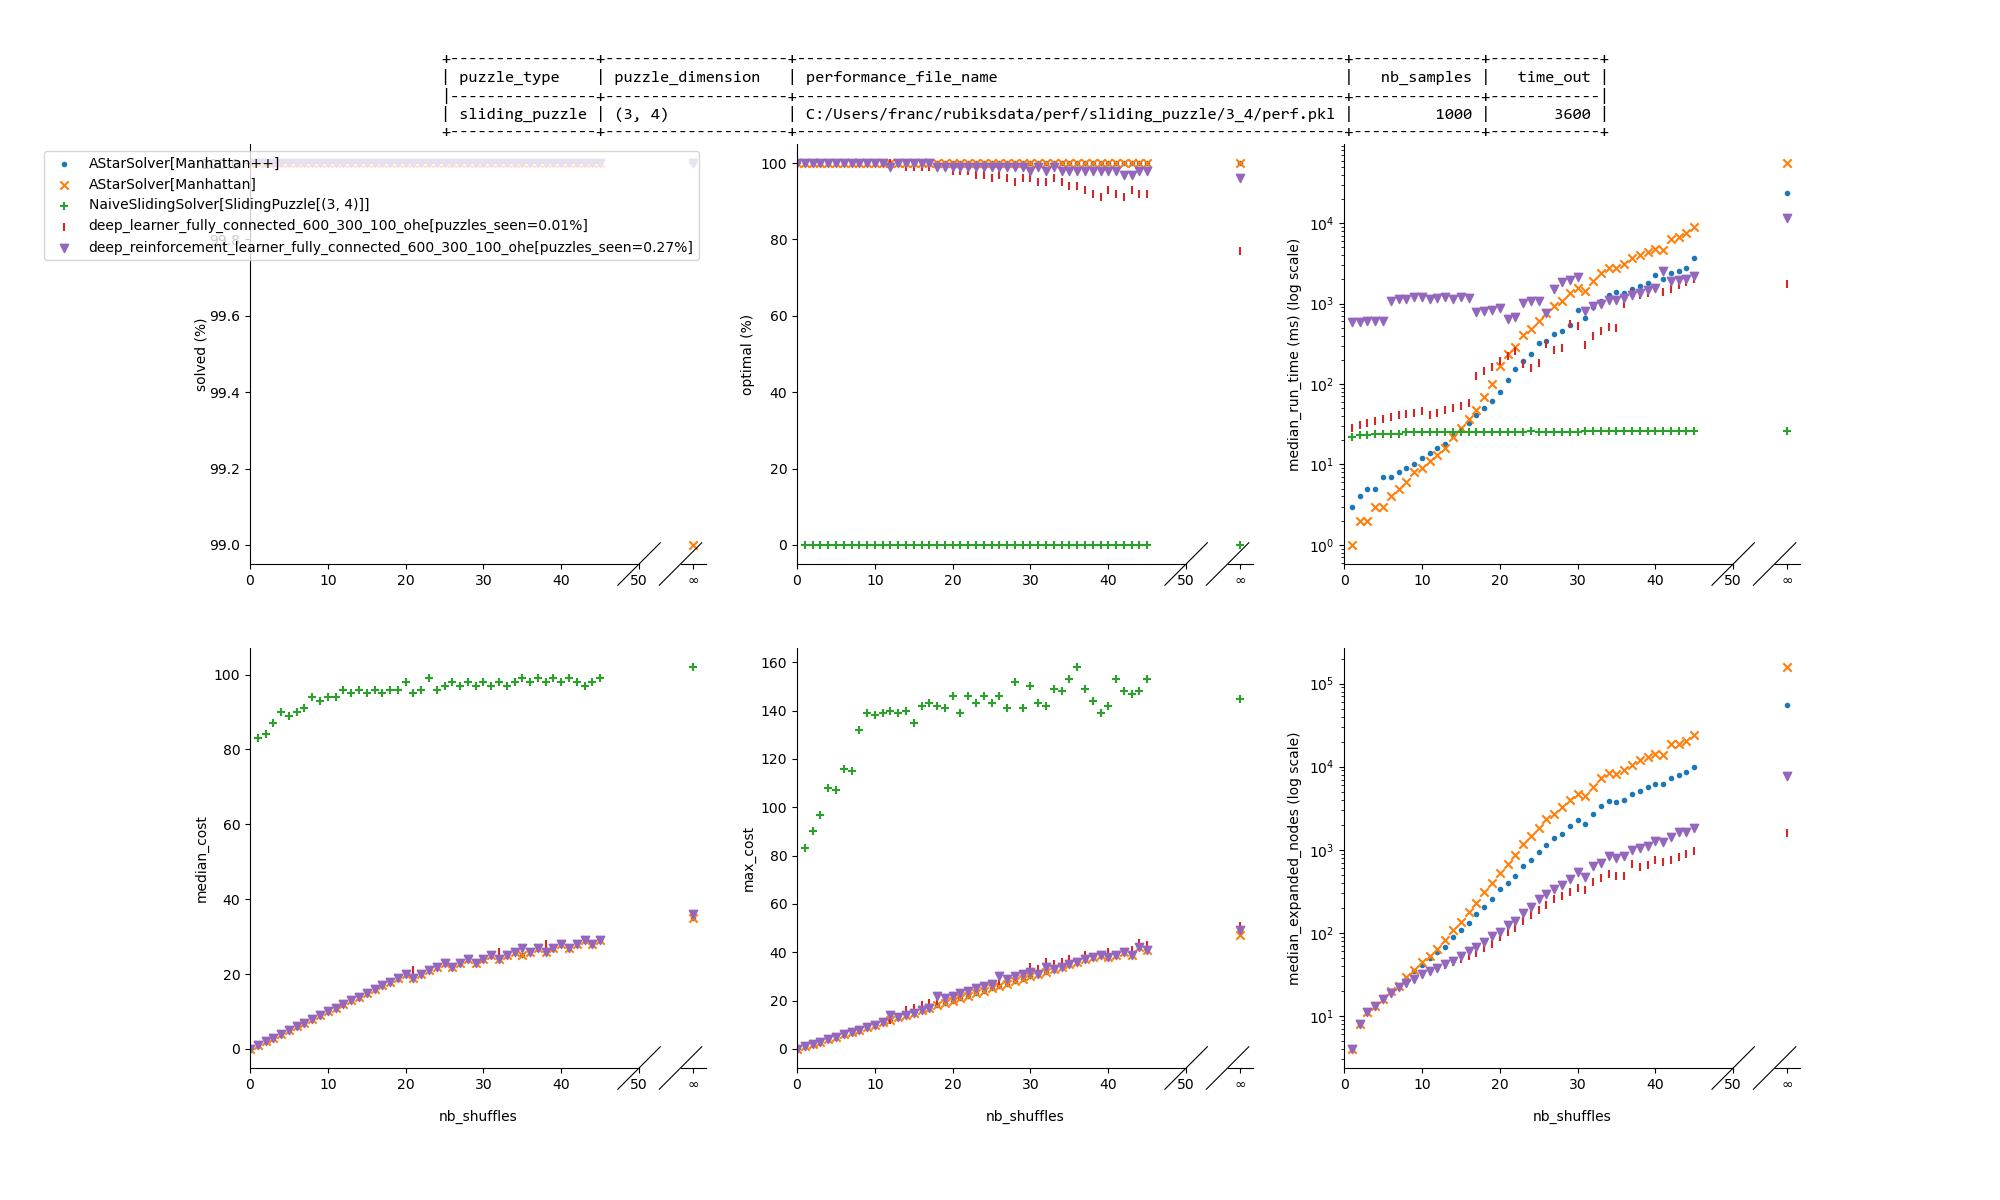
\includegraphics[scale=0.63]{./Figures/34SPPerformance.jpeg}
%\decoRule
\caption[34SPPerformance]{Solvers' performance comparison 3x4 SP}
\label{fig:34SPPerformance}
\end{figure}
\vfill
\end{landscape}
\restoregeometry
%-----------------------------------
%	SECTION 4
%-----------------------------------

\section{4x4}



\label{ssec:44SPSC}

\newgeometry{top=0mm, bottom=0mm, left=0mm, right=0mm}
\begin{landscape}
\centering\vspace*{\fill}
\begin{figure}[H]
\centering
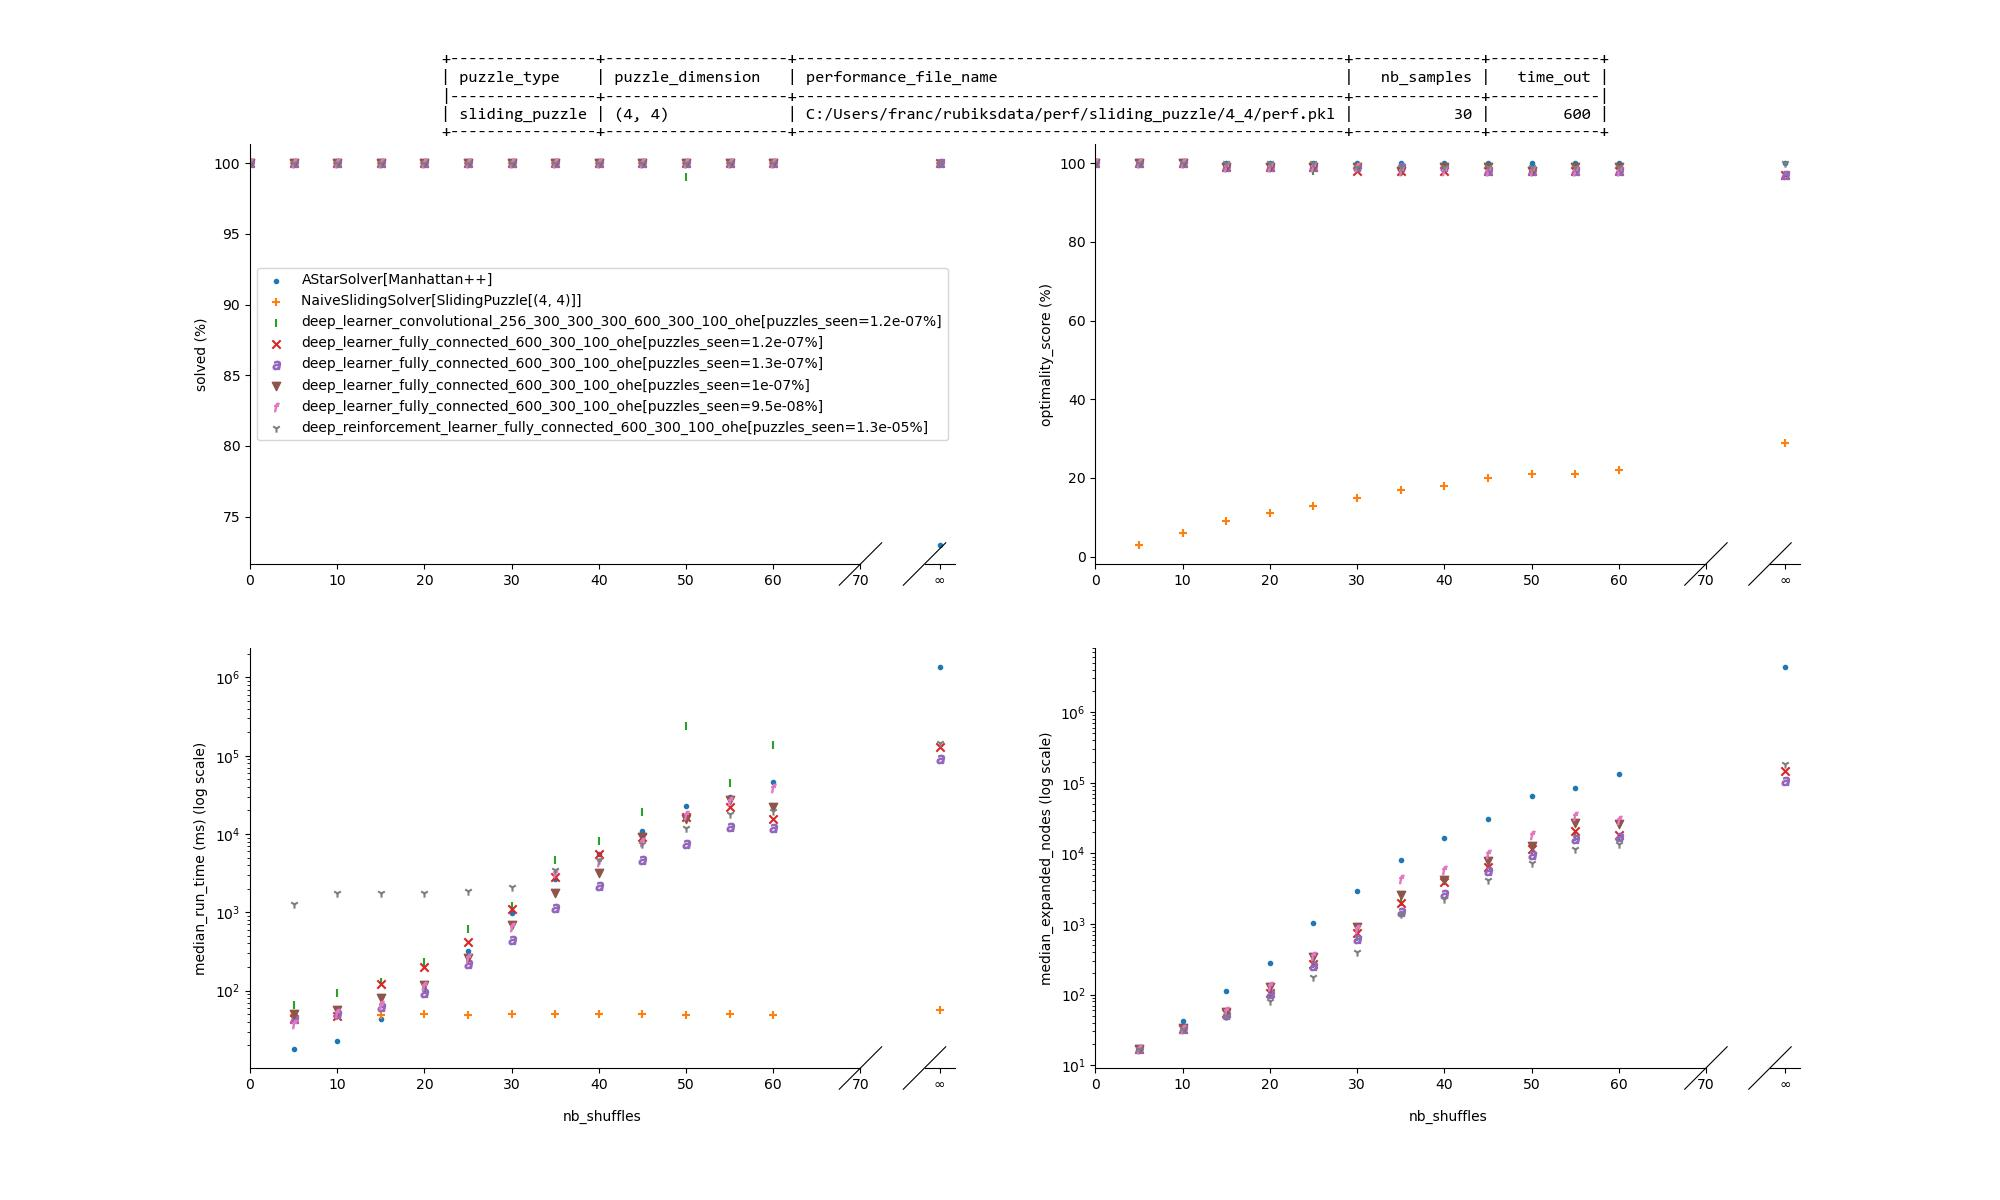
\includegraphics[scale=0.63]{./Figures/44SPPerformanceAll.jpeg}
%\decoRule
\caption[44SPPerformance]{Solvers' performance comparison 4x4 SP}
\label{fig:44SPPerformance}
\end{figure}
\vfill
\end{landscape}
\restoregeometry

%-----------------------------------
%	SECTION 5
%-----------------------------------

\section{5x5}

TBD

% Chapter Template

\chapter{Results - Rubik's Cube} % Main chapter title

\label{sec:ResRubiks} % Change X to a consecutive number; for referencing this chapter elsewhere, use \ref{ChapterX}

%----------------------------------------------------------------------------------------
%	SECTION 1
%----------------------------------------------------------------------------------------

In this second results section, I discuss my experiments on the Rubik's cube. I have run reasonably comprehensive experiments on the 2x2x2, throwing 6 of my solvers at the problem. As mentioned in \ref{sec:Puzzles}, the 2x2x2 \textbf{RC}, in spite of its deceivingly simple physical appearance, is actually not that much easier to solve (by hand) than the 3x3x3. For instance, it takes me usually just under 1 minute, wherras the 3x3x3 takes me only double that time, just under 2 minutes. I am obviously a beginner in Rubik's cube handsolving, but my personal ratio of time-to-solve and perceived difficulty is in line with that of experienced speedcubers who might take and average of, say, 2-3 seconds for the 2x2x2 and 10 seconds for the 3x3x3.
\\
Computing wise, the 2x2x2 was of decent size for my purpose, with its 88 million configurations. Let me start with a table summarizing which solvers I have attempted to run on the 2 dimensions I have attempted to experiment with:

\begin{center}
\begin{tabular}{l*{5}{c}r}
\hline
\textbf{solver}      & & \textbf{Rubik's} & \textbf{2x2x2} & \textbf{3x3x3} \\
\hline
BFS   &   &        &  x  &  x  \\
\hline
Kociemba   &   &      &  x  &  x  \\
\hline
A$^{*}$[Kociemba]  &   &  &  x  &  x  \\
\hline
A$^{*}$[DL[A$^{*}$[Kociemba]]]  &   &  &  x  &  x  \\
\hline
A$^{*}$[DRL]  &   &  &  x  &  \\
\hline
A$^{*}$[DQL]  &   &  &  x  &  \\
\hline
%MCTS[DQL][c=0]  &   &  & x &  \\
%\hline
%MCTS[DQL][c=69]  &   & & x &  \\
%\hline
\end{tabular}
\end{center}








\Section{2x2x2}
All the following experiments on the 2x2x2 \textbf{RC} have been run using my Solver's \textit{performance\_test} (see \ref{sec:codesolvers}): for each level of difficulty, the test present the solvers with the same 100 random configurations (for fairness and to increase the significance of the results). The levels of difficulty (number of scrambles from goal) used here go from 2 to 20 in step of 2. The tests were also run with perfect shuffling (difficulty = $\infty$ on the graphs), corresponding to taking scrambling to $\infty$ as explained in \ref{Theory:222RCSSS}).

\Subsection{BFS}
BFS is the only one for which I used a step of 1 on the difficuly and stopped at 5 as it was clear it would not go any further. Given that the run time and expanded nodes are clearly going to increase linearly, and given where 5 scrambling from goal took this solver already, there was no point going any further!

\Subsection{Kociemba, A$^{*}$[Kociemba], A$^{*}$[DL[A$^{*}$[Kociemba]]]}
Next, let me discuss Kociemba (see \cite{HKociemba} and \cite{Kociemba}) and associated experiments. We obviously expect Kociemba to be by far the fastest solver since it is handcrafted with much specific knowledge about the Rubik's cube group theory and multi-stage solving which I discussed in \ref{Theory:RCMSS}. I found the 2x2x2 library I used to not be optimal however, despite claims to the contrary. I have not had the time to investigate why this was not the case, but empirically I found that for instance running A$^{*}$ with Kociemba's cost as a heuristic was resulting in higher quality (i.e. of lower cost) solutions, clearly showing the non-optimality of Kociemba to begin with.
\\
\noindent Similarly to the higher dimensions \textbf{SP} from the previous section, there was no hope for me to run a perfect solver on the 2x2x2 \textbf{RC}. For starter, I have no admissible heuristic to guarantee optimality! Even if I had found one such heuristic and managed to implement it, it is doubtful I could have solved all 88 millions configurations without considerable work and time to reduce the configurations via symmetry arguments. As a result, I used solutions from A$^{*}$[Kociemba] on (perfectly) randomly generated configurations to train my \textbf{DL} heuristic. Thinking of it, it is rather amusing since Kociemba is itself using a two-stage IDA$^{*}$ solver, so I end-up here with 3 levels of nested A$^{*}$ algorithms, namely A$^{*}$[DL[A$^{*}$[IDA$^{*}$[2-stage-subgroups]]]].
\\
Notice finally that, since I have no optimal solver for the \textbf{RC}, I have set Kociemba as my benchmark in the performance test for the purpose of computing the optimality score. This is why some (actually all) of the other solvers will show scores larger than 100\% (top-right graph of figure \ref{fig:222RCPerformance}).






\Subsection{Deep Reinforcement Learner \& Deep Q Learner}
\label{sec:S33DRL}
To get my \textbf{DRL} and \textbf{DQL} heuristics, I have run the DeepReinforcementLearner and DeepQLearner with the following main parameters:
\begin{itemize}
\item Update the target network every 1,000 epochs (\textit{update\_target\_network\_frequency=1000}) or when the MSE falls below 10 basis points of the maximum target cost-to-go (\textit{update\_target\_network\_threshold=1e-3})
\item Run for a maximum of 11,000 epochs (\textit{nb\_epochs=11000}) or when the maximum target so far has not been increasing by more than 1\% in the last 5,500 epochs (\textit{max\_target\_uptick=1e-2} and \textit{max\_target\_not\_increasing\_epochs\_pct=0.5})
\item At every update of the target network (\textit{training\_data\_every\_epoch=False}), generate 10,00 sequences of puzzles (\textit{nb\_sequences=10,000}), each comprised of a 15-scramble puzzle back to goal state, with all intermediary puzzles along the path (\textit{nb\_shuffles=15}).
\item Use a fully connected network (\textit{network\_type=fully\_connected\_net}) with three hidden layers of size 600, 300, 100 (\textit{layers\_description=(600,300,100)}) and use torch.optim.RMSProp as optimiser (\textit{optimiser=rms\_prop}) with an exponential scheduler (\textit{scheduler=exponential\_scheduler}) with gamma 0.999 (\textit{gamma\_scheduler=0.9999}) and \textit{learning\_rate=0.001}. The networks architecture is shown in figure \ref{fig:222RCnets}.
\end{itemize}
Graphs \ref{fig:222RCDRL} and \ref{fig:222RCDQL} show both learners' following metrics tracked over the epochs:
\begin{itemize}
\item learning rate, which decreases due to the scheduler, but gets reset at each network update.
\item max target. One interesting dynamic during learning is that due to the way targets are constructed using value-iteration update, and starting from an all 0 network, the max target only increases by about 1 at best at every network update. That is, the first network only learns how to differentiate goal from non-goal, then the second one learns how to differentiate goals, cost 1 and cost 2+ in some sense. This is why I have introduced the first set of parameters discussed just above. The first one makes sure we do not waste time initially training the left-hand-side network when training is easy (as consist of just goal versus not goal). The second ones make sure that we stop training altogether when the max target does not grow anymore. This is because we do not know a-priori what the God number of a given puzzle/dimension is, but let's assume for the sake of the argument that it is 15. Then that means that after 15 updates of the target network we might not really get so much benefit by keeping training and value-iterating.
\item the loss (MSE for \textbf{DRL}, MSE + CrossEntropyLoss for \textbf{DQL})
\item the loss divided by the max target. The exit criterion \textit{update\_target\_network\_threshold} is based on that quantity, since a loss of e.g. 0.01 means little if the we do not compare it to the possible range that the cost-to-go can take.
\item The percentage of all the possible puzzles of that dimension \textit{seen} by the DeepReinforcementLearner. This is an interesting quantity, as it tells us later on when testing out of sample and comparing with other solvers, how well the solvers are able to generalise. In this case (3x3) we can see that the DeepReinforcementLearner quickly has seen a very large percentage of all puzzles. That being said, it is good to keep in mind that \textit{seen} does not mean really much here, since the learning is unsupervised. This is quite in contrast to the DeepLearner, for which puzzles seen come along with the cost-to-go computed by a \textit{teacher}, usually an optimal or at least efficient solver.
\end{itemize}


\begin{figure}
  \noindent
  \makebox[\textwidth]{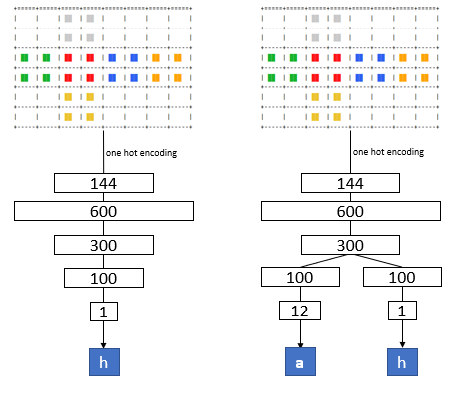
\includegraphics[scale=0.6]{./Figures/222RCnets}}
  \caption[222RCnets]{2x2x2 \textbf{RC} architecture for \textbf{DRL} (left) \& \textbf{DQL} (right) heuristics training}
  \label{fig:222RCnets}
\end{figure}


\begin{figure}
  \noindent
  \makebox[\textwidth]{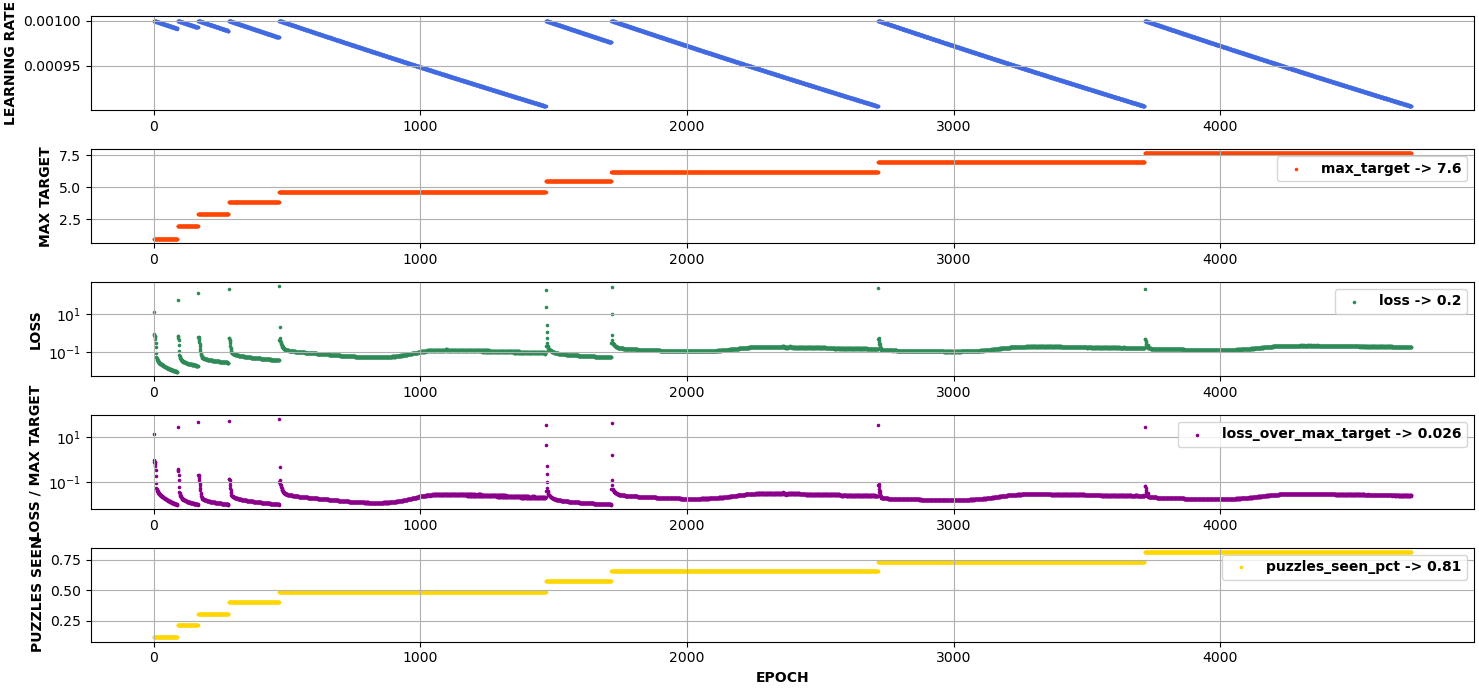
\includegraphics[scale=0.5]{./Figures//222RCDRL}}
  \caption[222RCDRL]{\textbf{DRL} of the 2x2x2 \textbf{RC}}
  \label{fig:222RCDRL}
\end{figure}

\begin{figure}
  \noindent
  \makebox[\textwidth]{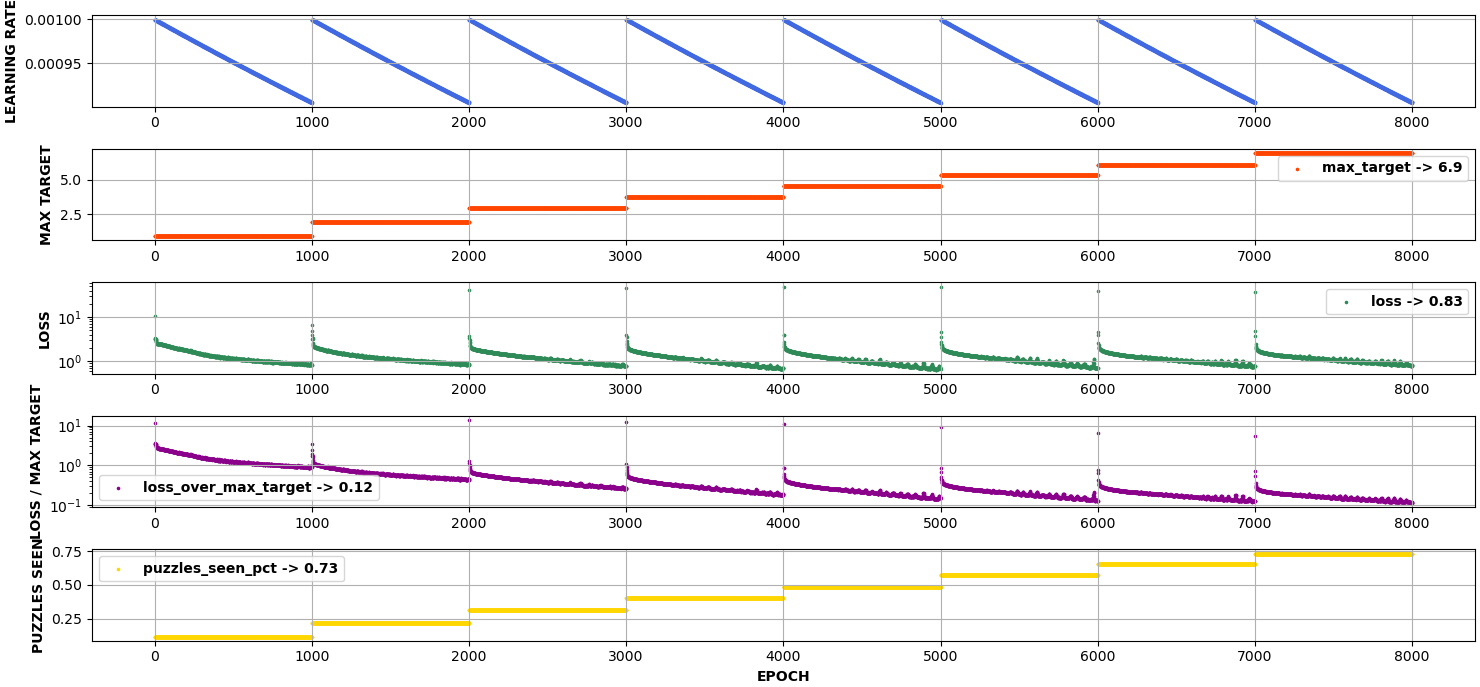
\includegraphics[scale=0.5]{./Figures//222RCDQL}}
  \caption[222RCDQL]{\textbf{DQL} of the 2x2x2 \textbf{RC}}
  \label{fig:222RCDQL}
\end{figure}




\Subsection{Solvers' comparison}

We summarize as usual the 2x2x2 \textbf{RC} performance tests by our usual metrics \ref{fig:222RCPerformance}. Overall, the \textbf{DL} and \textbf{DRL} managed to solve all cubes (though \textbf{DL} took over an houd and \textbf{DRL} up to 6 hours for the slowest cube they encountered. Both methods outperformed in terms of optimality score Kociemba and got on par with A$^{*}[Kociemba]$. Their max cost over all cubes encountered was 12 for up to 20 shuffles, and 13 for $\infty$ shuffling. Considering God's number for the 2x2x2 \textbf{RC} of 11, this is rather impressive!
\\
\\
An very interesting remark is that if we check the learning graph \ref{fig:222RCDRL} of the \textbf{DRL}, we can see it only ever assigned a cost-to-go (value function) of 7.6 at most. Despite that fact, it was still able to solve cubes requiring 13 moves. How is that possible? Notice that the loss of 0.2 towards which it converged at the end of its training is misleading, since it is not a loss versus the actual true cost-to-go, but rather versus that of the target network. My theory is that while the value the \textbf{DRL} assigned to hard-to-solve cubes is off (by at least 4 or 5), it is likely the case that the network gets the relative value of neighbouring cubes about right, and this is sufficient to guide A$^{*}$ extremely well.
\\
\\
Finally, we can see that \textbf{DQL}, despite showing seemingly/visually cleaner and more monotonic loss convergence than \textbf{DRL} (see \ref{fig:222RCDQL} versus \ref{fig:222RCDRL}), struggled a lot more to solve difficult cubes (above 10 shuffles). Clearly this shows that my earlier findings on the 3x3 \textbf{SP} are likely not universal, and very much depend on the parameters set during training, as well as on the problem at hand.

\begin{figure}[H]
  \noindent
  \makebox[\textwidth]{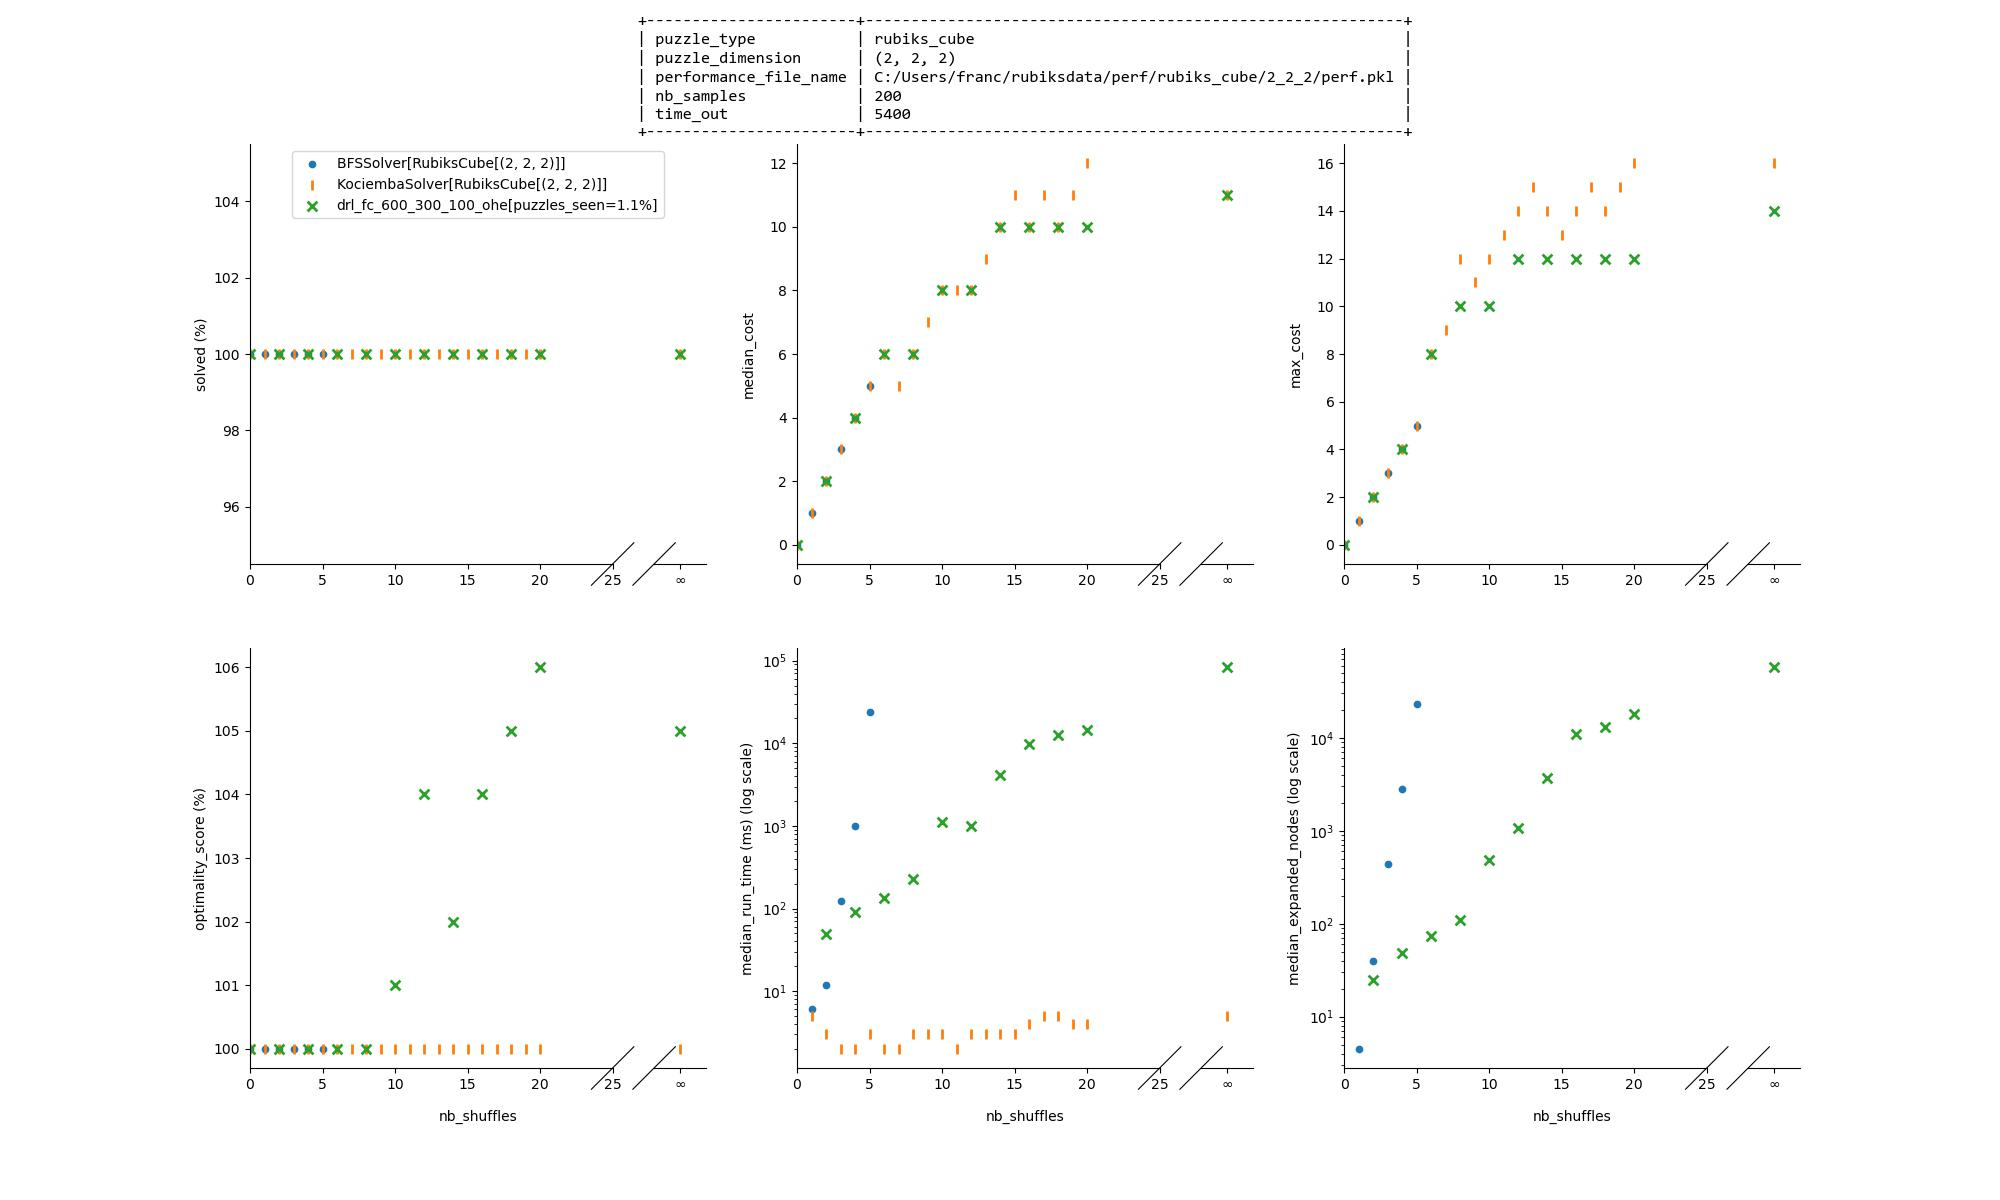
\includegraphics[scale=0.55]{./Figures/222RCPerformance}}
  \caption[222RCPerformance]{Solvers' performance comparison 2x2x2 \textbf{RC}}
  \label{fig:222RCPerformance}
\end{figure}



%-----------------------------------
%	SUBSECTION 1
%-----------------------------------
\Section{3x3x3}
\label{sec:ResRubiks333}

I did not get to run very many experiments on the 3x3x3 \textbf{RC}. The results of the performance test (50 random configurations for levels of difficulty from 2 to 40 by increment of 2 as well as $\infty$ shuffling) can be found on figure \ref{fig:333RCPerformance}.
\begin{itemize}
\item Here again, Kociemba does not show optimality, since we can see that my A$^{*}[Kociemba]$, that is A$^{*}$ using Kociemba as a heuristic, performs much better than Kociemba (solutions about 20\% shorter at $\infty$ shuffling). This is not surprising though since Kociemba 3x3x3 does not claim to be optimal and is meant to find solution in the 40 moves at most (which is what I have observed indeed). A$^{*}[Kociemba]$ never took more than 30 moves on any of the cubes presented to it, which is not bad given the known God number of 26 in the quarter-turn-metric (as discussed earlier in \ref{Theory:333RCSSS})
\item A$^{*}$[\textbf{DL}] managed to solve all puzzles scrambled less than 10 times, and found shorter worst case solutions than even A$^{*}[Kociemba]$ on which it was trained. Within the 2 hours time out, it failed to solve one of the 50 cubes for difficulty 10, and two of the 50 cubes of difficulty 12, so i did not try further than that.
\item A$^{*}$[\textbf{DRL}] only managed to solve all puzzles of difficulty less than 6 but at least did find only optimal solutions (compared with \textbf{BFS}).
\end{itemize}


\begin{figure}[H]
  \noindent
  \makebox[\textwidth]{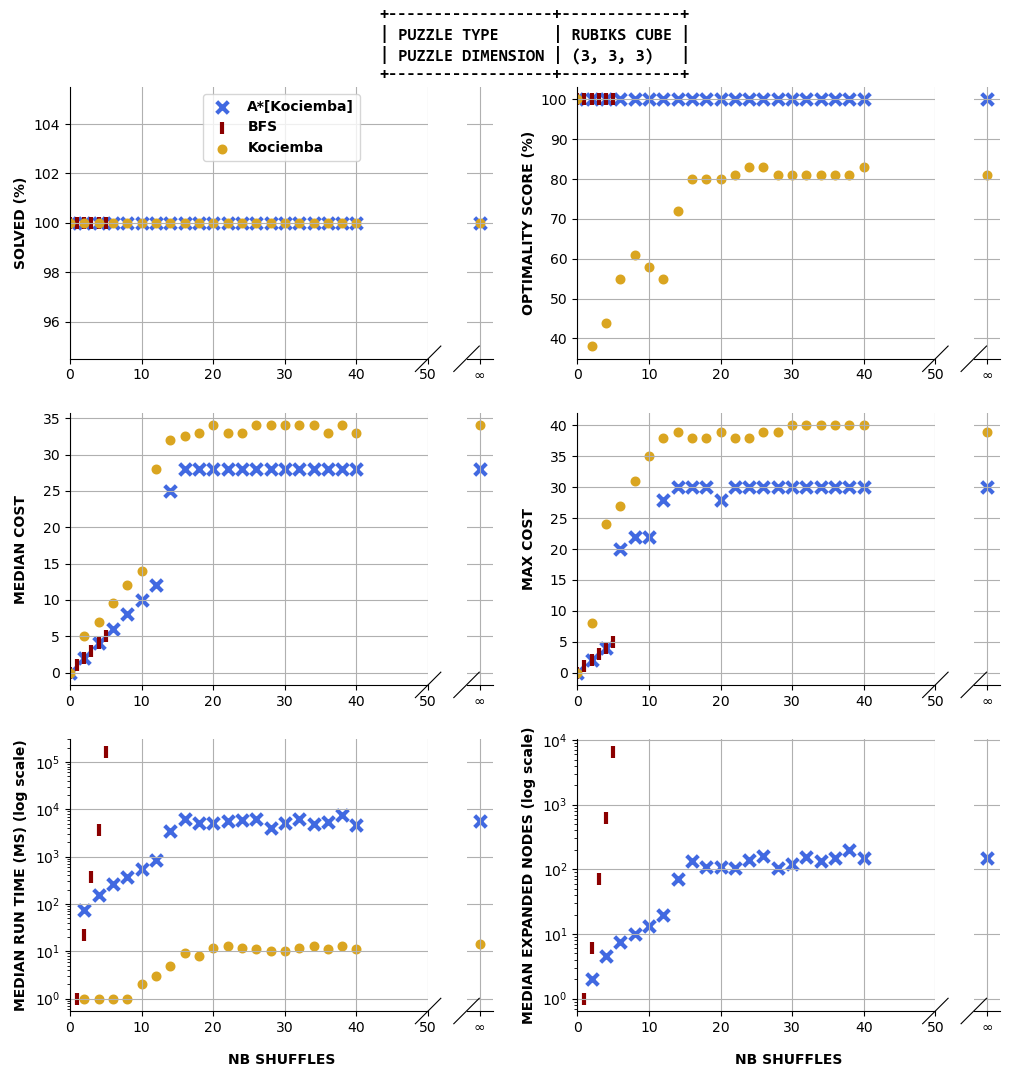
\includegraphics[scale=0.55]{./Figures/333RCPerformance}}
  \caption[333RCPerformance]{Solvers' performance comparison 3x3x3 \textbf{RC}}
  \label{fig:333RCPerformance}
\end{figure}


%----------------------------------------------------------------------------------------
%	THESIS CONTENT - APPENDICES
%----------------------------------------------------------------------------------------

\appendix % Cue to tell LaTeX that the following "chapters" are Appendices

% Include the appendices of the thesis as separate files from the Appendices folder
% Uncomment the lines as you write the Appendices

%% Appendix A

\chapter{Frequently Asked Questions} % Main appendix title

\label{AppendixA} % For referencing this appendix elsewhere, use \ref{AppendixA}

\section{How do I change the colors of links?}

The color of links can be changed to your liking using:

{\small\verb!\hypersetup{urlcolor=red}!}, or

{\small\verb!\hypersetup{citecolor=green}!}, or

{\small\verb!\hypersetup{allcolor=blue}!}.

\noindent If you want to completely hide the links, you can use:

{\small\verb!\hypersetup{allcolors=.}!}, or even better: 

{\small\verb!\hypersetup{hidelinks}!}.

\noindent If you want to have obvious links in the PDF but not the printed text, use:

{\small\verb!\hypersetup{colorlinks=false}!}.

%\include{Appendices/AppendixB}
%\include{Appendices/AppendixC}

%----------------------------------------------------------------------------------------
%	BIBLIOGRAPHY
%----------------------------------------------------------------------------------------


%\begin{thebibliography}{widest entry}

%\bibitem{sliddingpuzzle} Whatever
%{\href{https://en.wikipedia.org/wiki/Sliding\_puzzle}{wikipedia}} Sliding Puzzle Wikipedia article, accessed 19th June 2022

%\end{thebibliography}


%\printbibliography[heading=bibintoc]
\printbibheading
\printbibliography[type=article,heading=subbibliography,title={Journal Papers}]
\printbibliography[type=book,heading=subbibliography,title={Books}]
\printbibliography[type=misc,heading=subbibliography,title={Misc}]

%----------------------------------------------------------------------------------------

\end{document}  
